\documentclass[10pt]{article}
\usepackage{blindtext}
\usepackage{amsfonts}
\usepackage{graphicx}
\usepackage{array}
\setlength{\parindent}{0em}
\newcolumntype{P}[1]{>{\centering\arraybackslash}p{#1}}
\graphicspath{ {/Users/Xiaopei/Documents/Coursework/Fall\ 2017/STATS\ M231/Project\ 2/Report}}
\usepackage[margin=1in]{geometry}
\title{Project 2: Human Face Detection using Boosting}
\author{Xiaopei Zhang (004309991)}
\date{\today}
\begin{document}
\maketitle
\section*{\large{Task 1: Construct weak classifiers}}
	Load the predefined set of Haar filters. Compute the features $\{f_j\}$ by applying each Haar filter to the integral images of the positive and negative populations. Determine the polarity $s_j$ and threshold $\theta_j$ for each weak classifier $h_j$. Specifically, we consider 20 intervals for the threshold in this project. Write a function that achieves this. In each iteration of AdaBoost, the function returns the weak classifier with the lowest weighted error.\\ 
	
\section*{\large{Task 2: Implement AdaBoost}}
	Implement the AdaBoost algorithm to boost the weak classifiers. Construct the strong classifier $H(x)$ as a weighted ensemble of $T$ weak classifiers.\\\\
	(a) \textbf{Haar filters:} Figure 1 displays the visualization of top 20 Haar filters, as well as their voting weights, after boosting. These filters are selected using the function we write for Task 1 when $t=1,2,...,20$.\\
	\begin{figure}[ht]
		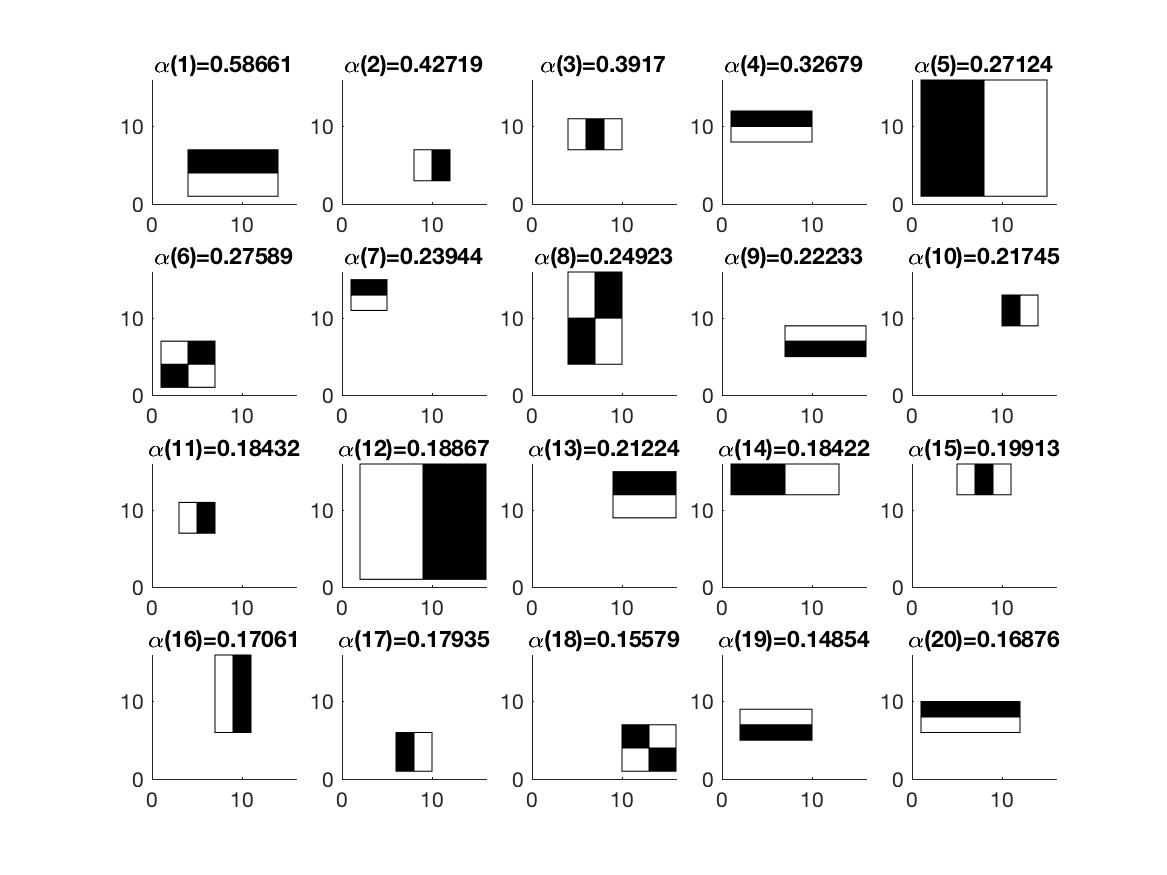
\includegraphics[scale = 0.25]{top_20_Haar_filter.jpg}
		\centering
		\caption{Top 20 Haar filters.}
		\label{1}
	\end{figure}\\
	(b) \textbf{Training error of strong classifier:} Figure 2 displays the plot of the training error of the strong classifier over the number of steps $T$. As we may notice, the overall training error decreases as the weak classifier boosting continues. Finally, our training error converges to around $0.06$, which is good enough.\\
	\begin{figure}[ht]
		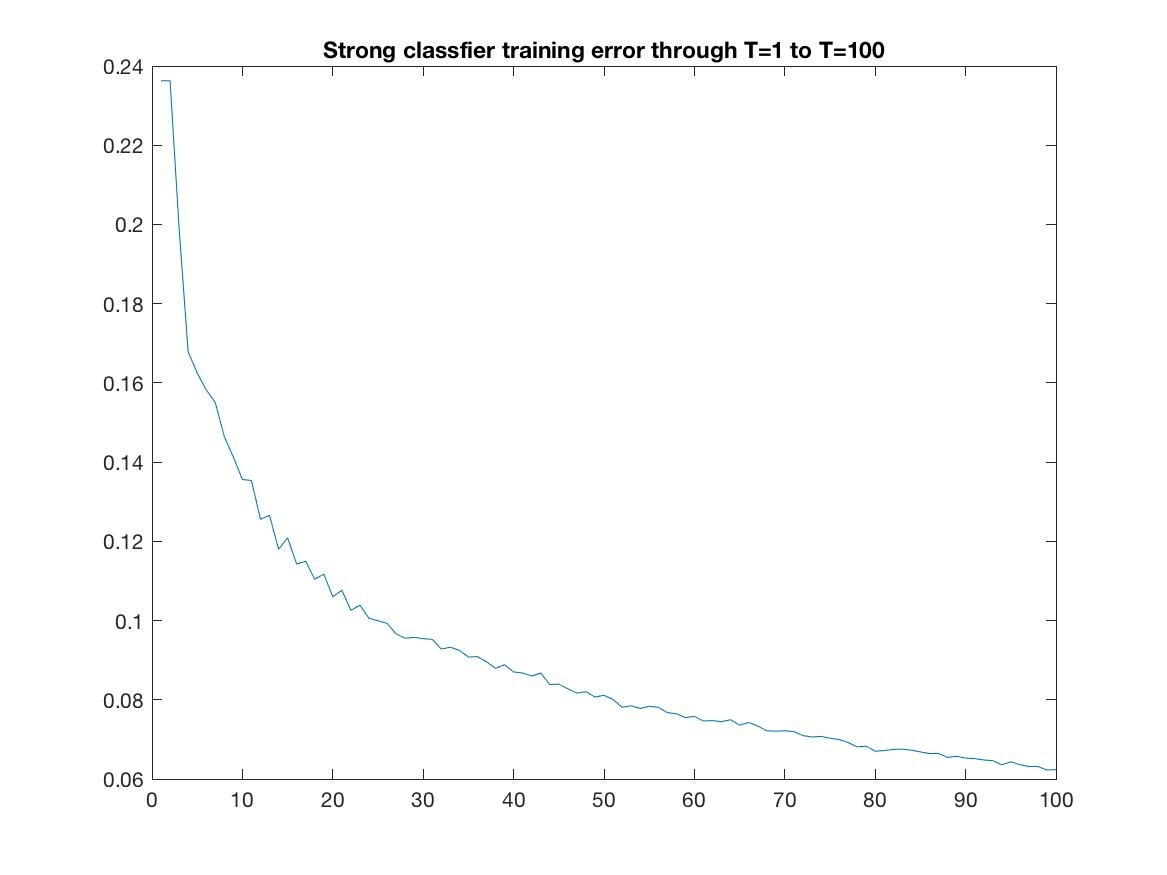
\includegraphics[scale = 0.25]{strong_classifier_training_error.jpg}
		\centering
		\caption{Training error of strong classifier over T.}
		\label{2}
	\end{figure}\\
	(c) \textbf{Training errors of weak classifiers:} Figure 3 shows the curve for the training errors of the top $1,000$ weak classfiers among the pool of weak classifiers in increasing order at $T=0,10,50,100$. From the figure, we realize that as $T$ increases, the performance of the best weak classifier becomes worse, but the overall performances of all weak classifiers become much more balanced, meaning that they achieves more similar training errors.\\
	\begin{figure}[ht]
		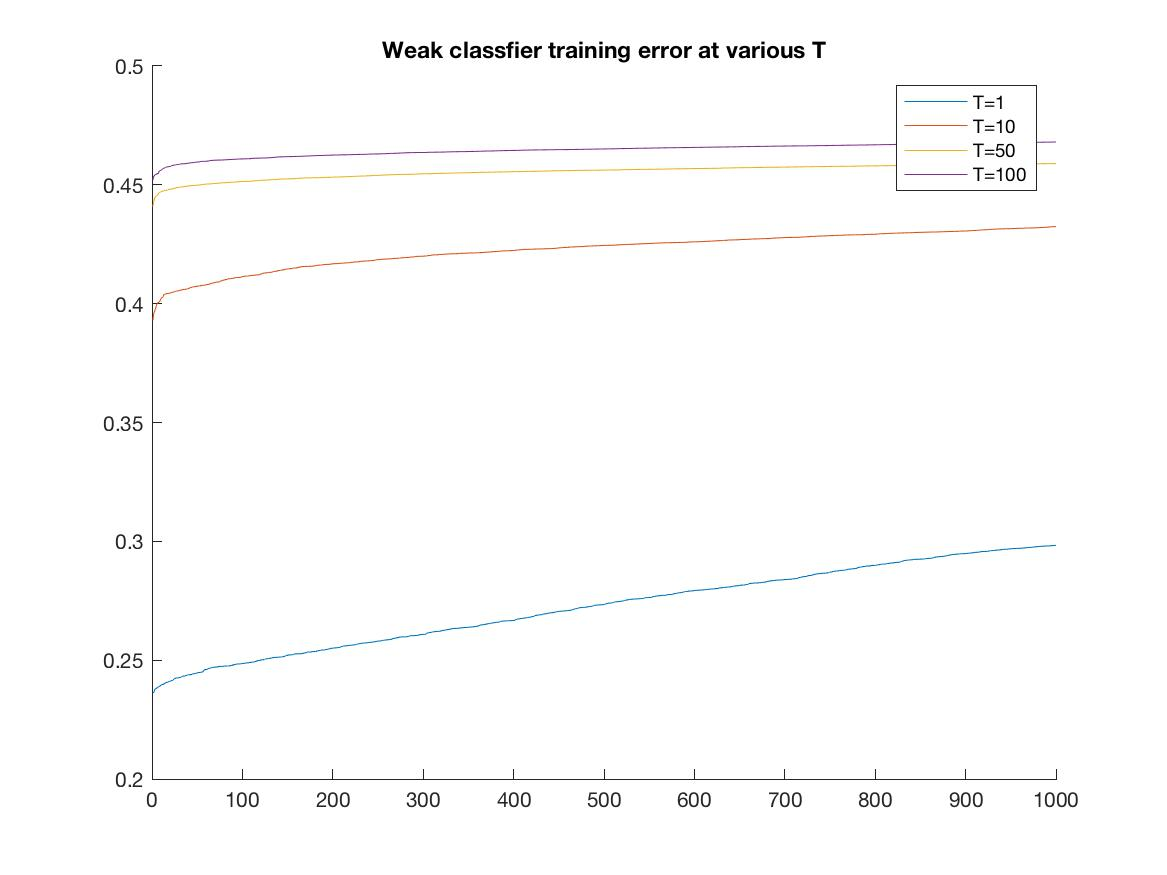
\includegraphics[scale = 0.25]{top_1000_weak_classifiers.jpg}
		\centering
		\caption{Weak classifier training error curves for $T=0,10,50,100$.}
		\label{3}
	\end{figure}\\
	(d) \textbf{Histograms:} Figure 4, 5, 6 display the histograms of the positive and negative populations over $F(x)$, for $T=10,50,100$, respectively. From these histograms, we observe that as the boosting process continues, the intersection of their distributions become smaller. That is, the positive and negative populations become more and more differentiable by our strong classifier.\\
	\begin{figure}[ht]
		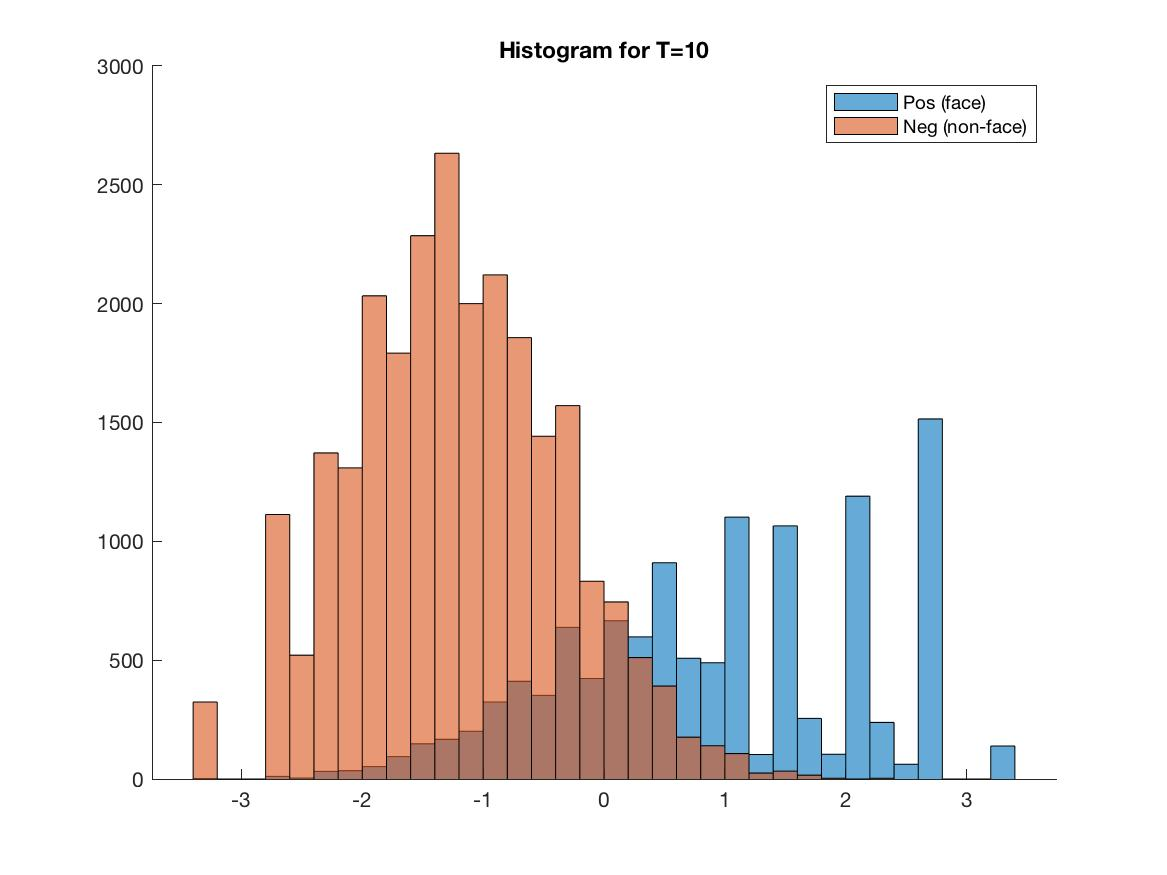
\includegraphics[scale = 0.2]{pos_neg_hist_10.jpg}
		\centering
		\caption{The positive and negative populations over $F(x)$ for $T=10$.}
		\label{4}
	\end{figure}
	\begin{figure}[ht]
		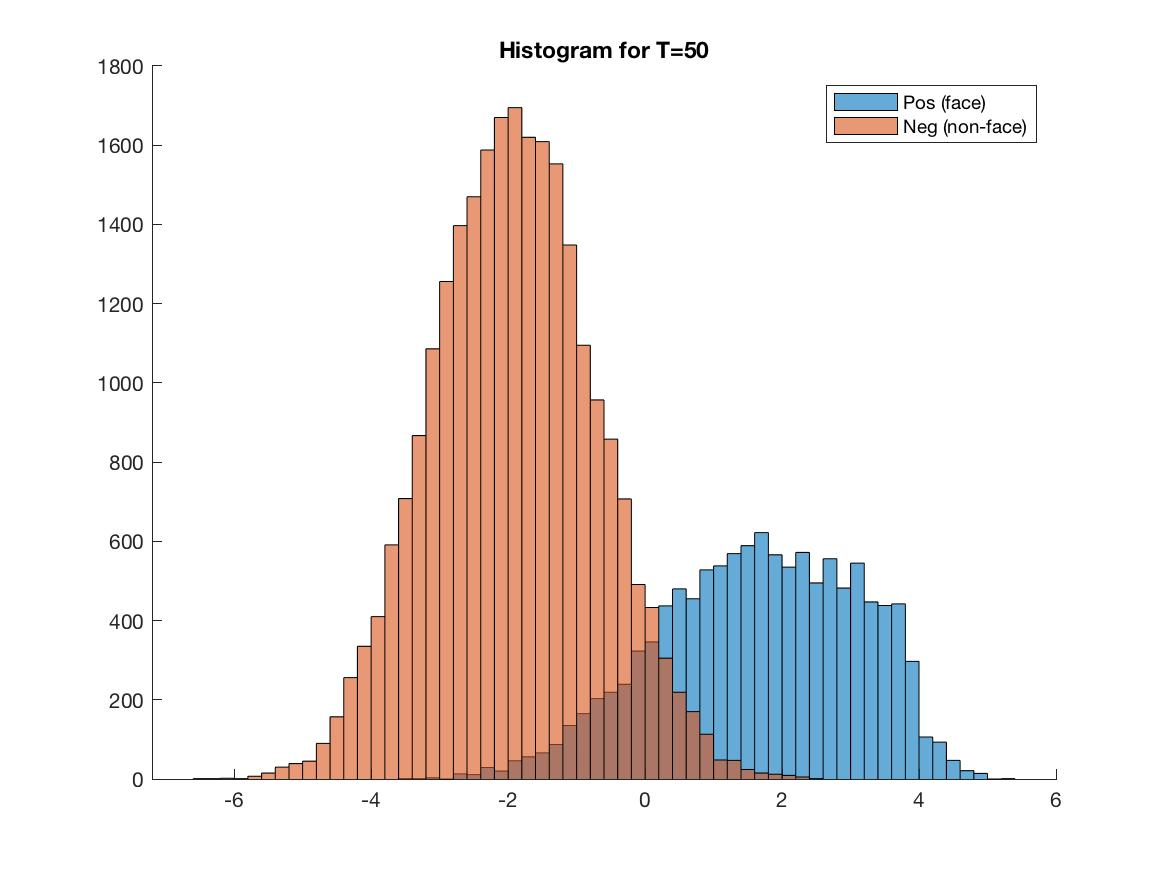
\includegraphics[scale = 0.2]{pos_neg_hist_50.jpg}
		\centering
		\caption{The positive and negative populations over $F(x)$ for $T=50$.}
		\label{5}
	\end{figure}
	\begin{figure}[ht]
		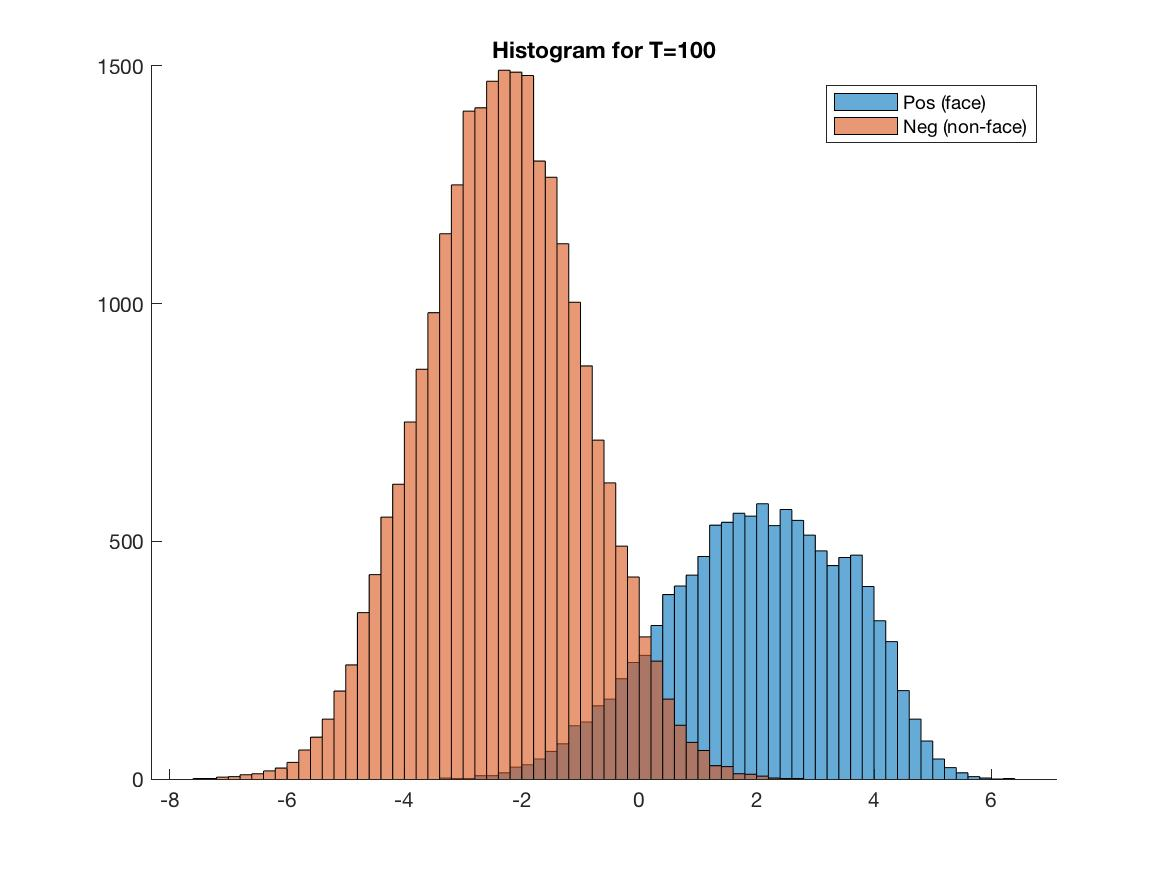
\includegraphics[scale = 0.2]{pos_neg_hist_100.jpg}
		\centering
		\caption{The positive and negative populations over $F(x)$ for $T=100$.}
		\label{6}
	\end{figure}\\
	\newpage(e) \textbf{ROC:} Figure 7 shows the corresponding ROC curves for the histograms of $T=10,50,100$ respectively. From the curve plot, we notice that as $T$ increases, the curve is much more uplifted toward the point $(0,1)$, where there are no false alarms as well as missing cases. Therefore, boosting is indeed effective.\\
	\begin{figure}[ht]
		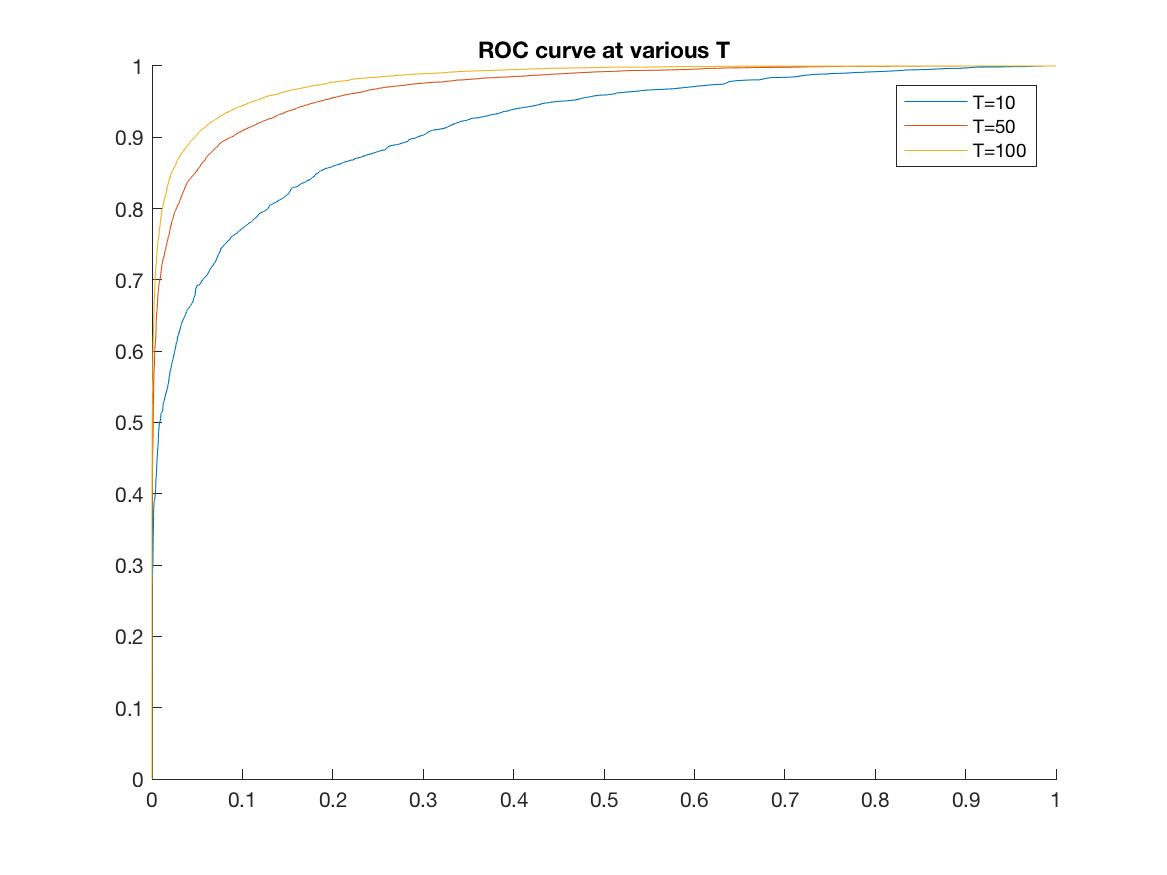
\includegraphics[scale = 0.25]{roc.jpg}
		\centering
		\caption{ROC curves for $T=10,50,100$.}
		\label{7}
	\end{figure}\\
	(f) \textbf{Detections:} Six class photos are given (three with people facing to the camera and three with people not facing to the camera). We scale each of them by $0.1\times2^f$, where $f=0.2k, k=0,1,...,20$, so that most of the faces would get a chance to fit in the $16\times16$ frame. Run our strong classifier derived after $T=100$. Perform non-maximum suppression with a permitted overlap of 0.05. Figure 8, 9, 10 display the detection results on positive sample images, from which we see that most faces are successfully detected, but there still exist some false alarms. Figure 11, 12, 13 display the detection results on negative sample images. The boxes detected in these figures (about 200 in total) will be used as hard negatives for hard negative mining in the next step. \\
	\newpage\begin{figure}[ht]
		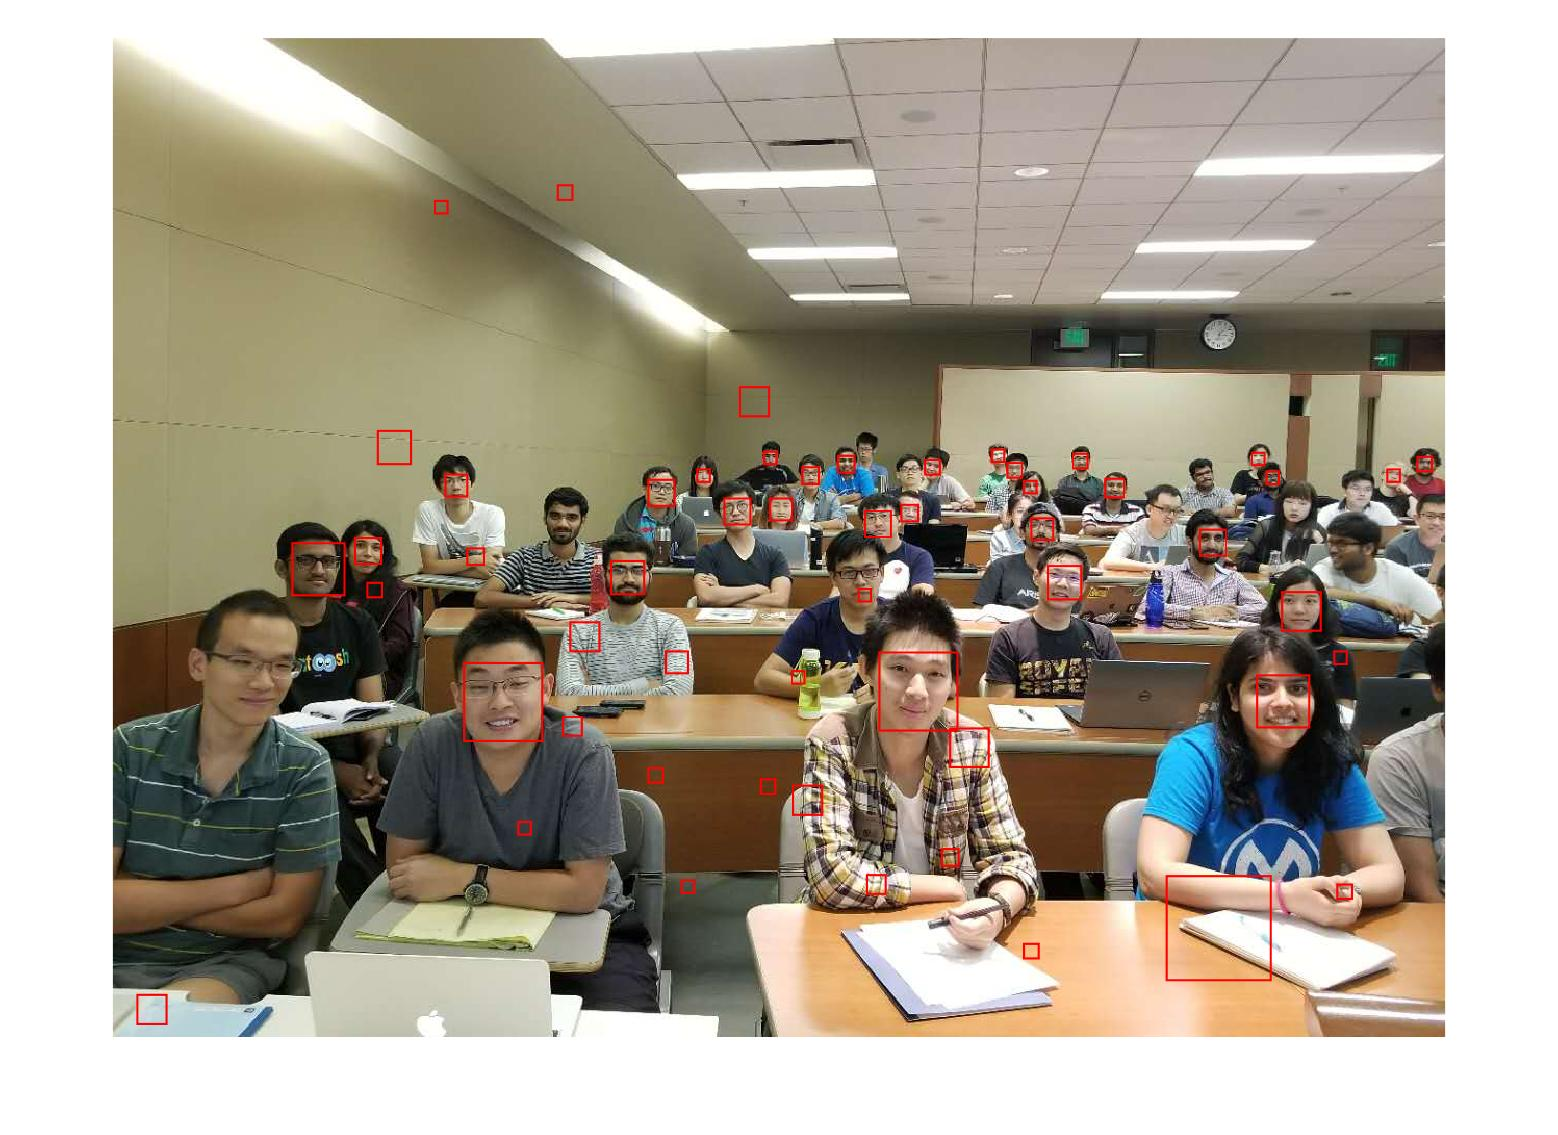
\includegraphics[width=\textwidth]{detection_face_1.jpg}
		\centering
		\caption{Detection result for positive sample image 1 without hard negative mining.}
		\label{8}
	\end{figure}
	\newpage\begin{figure}[ht]
		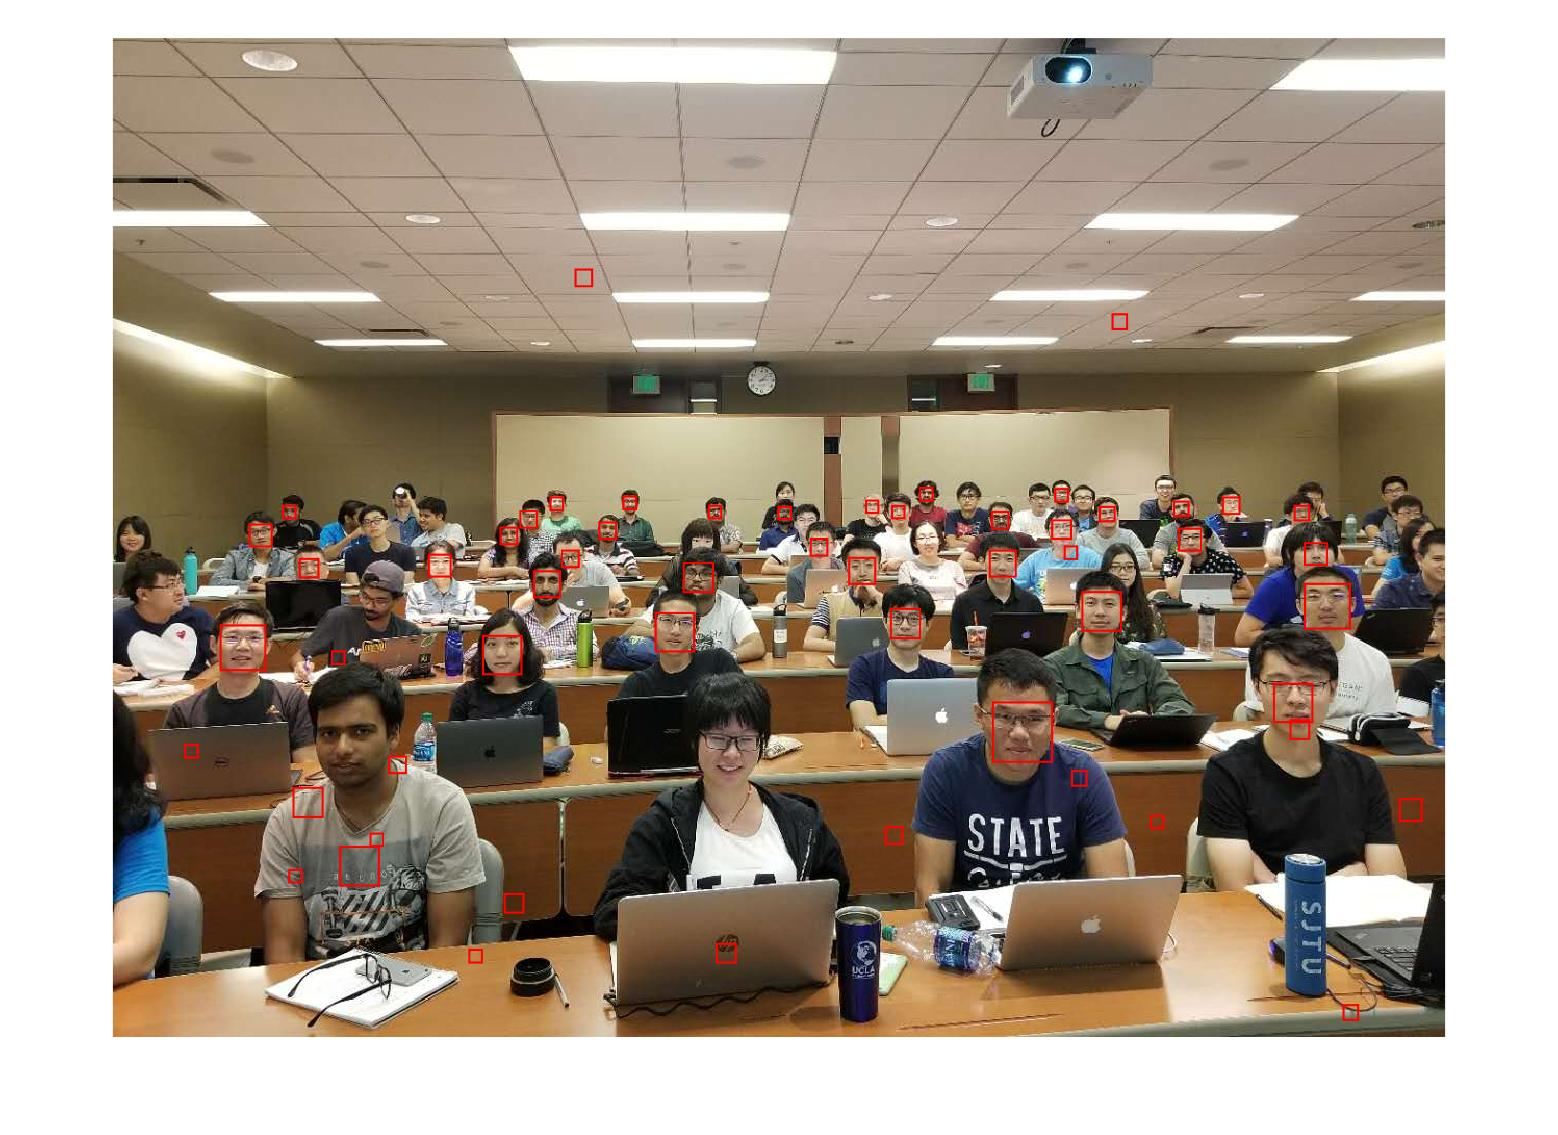
\includegraphics[width=\textwidth]{detection_face_2.jpg}
		\centering
		\caption{Detection result for positive sample image 2 without hard negative mining.}
		\label{9}
	\end{figure}
	\newpage\begin{figure}[ht]
		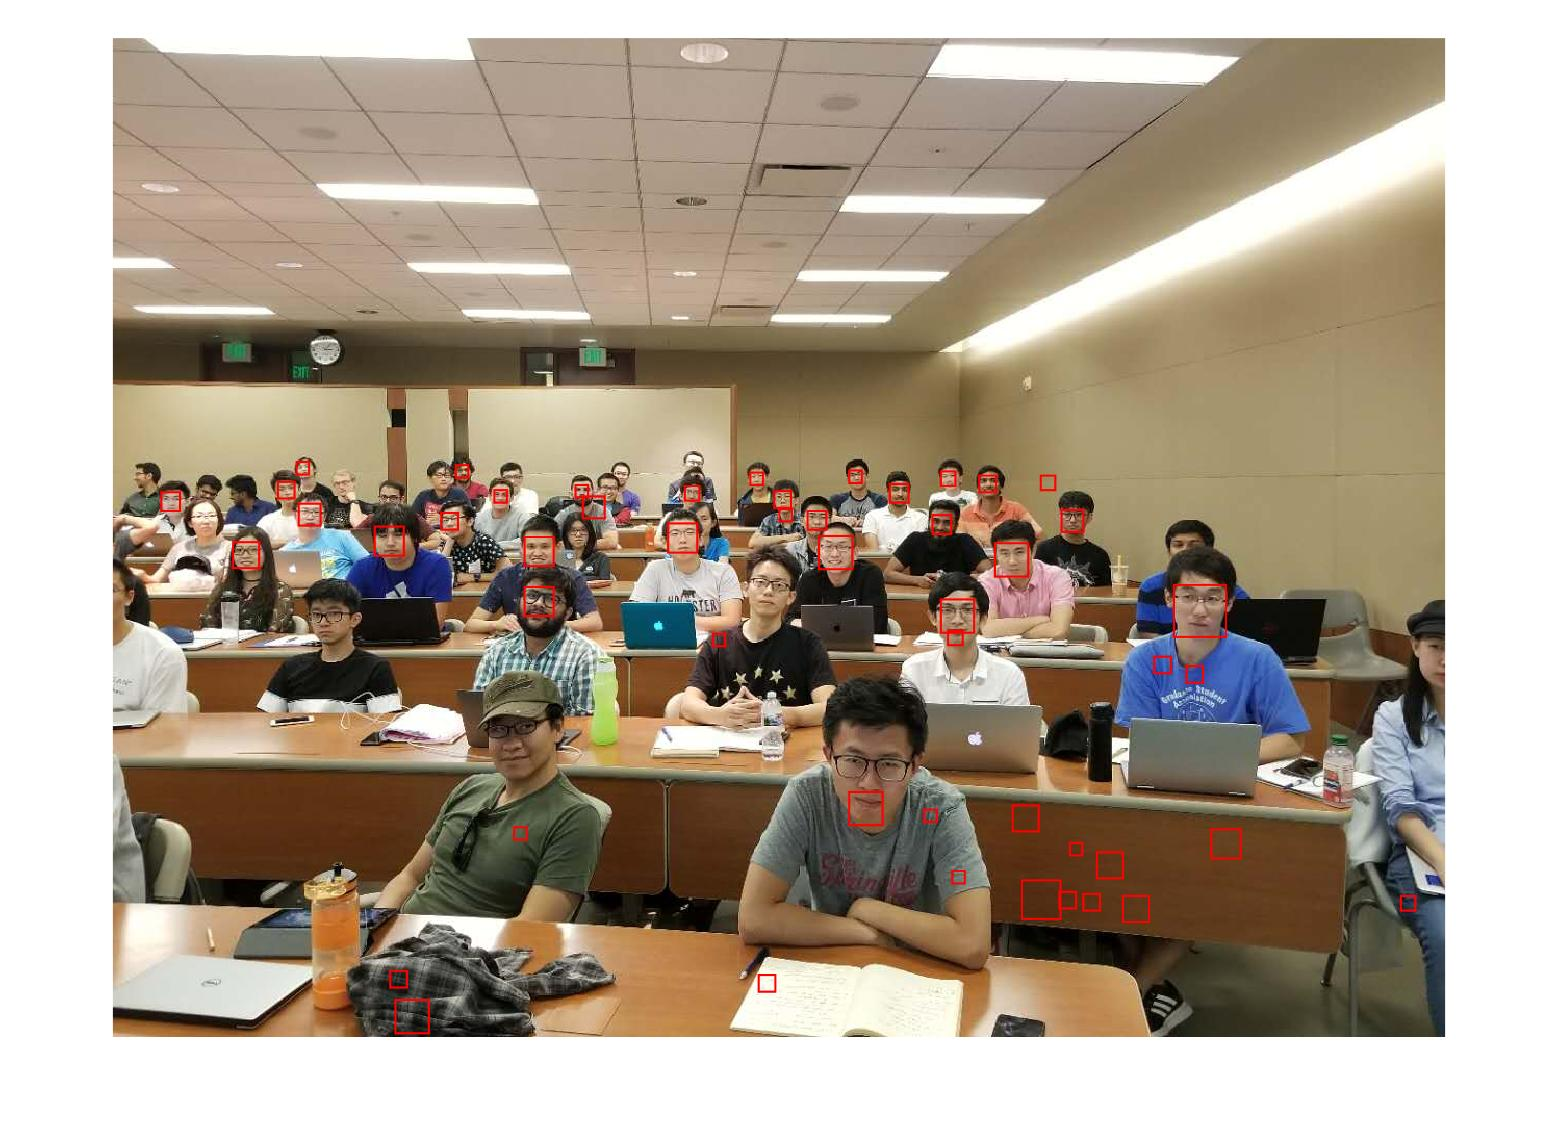
\includegraphics[width=\textwidth]{detection_face_3.jpg}
		\centering
		\caption{Detection result for positive sample image 3 without hard negative mining.}
		\label{10}
	\end{figure}
	\newpage\begin{figure}[ht]
		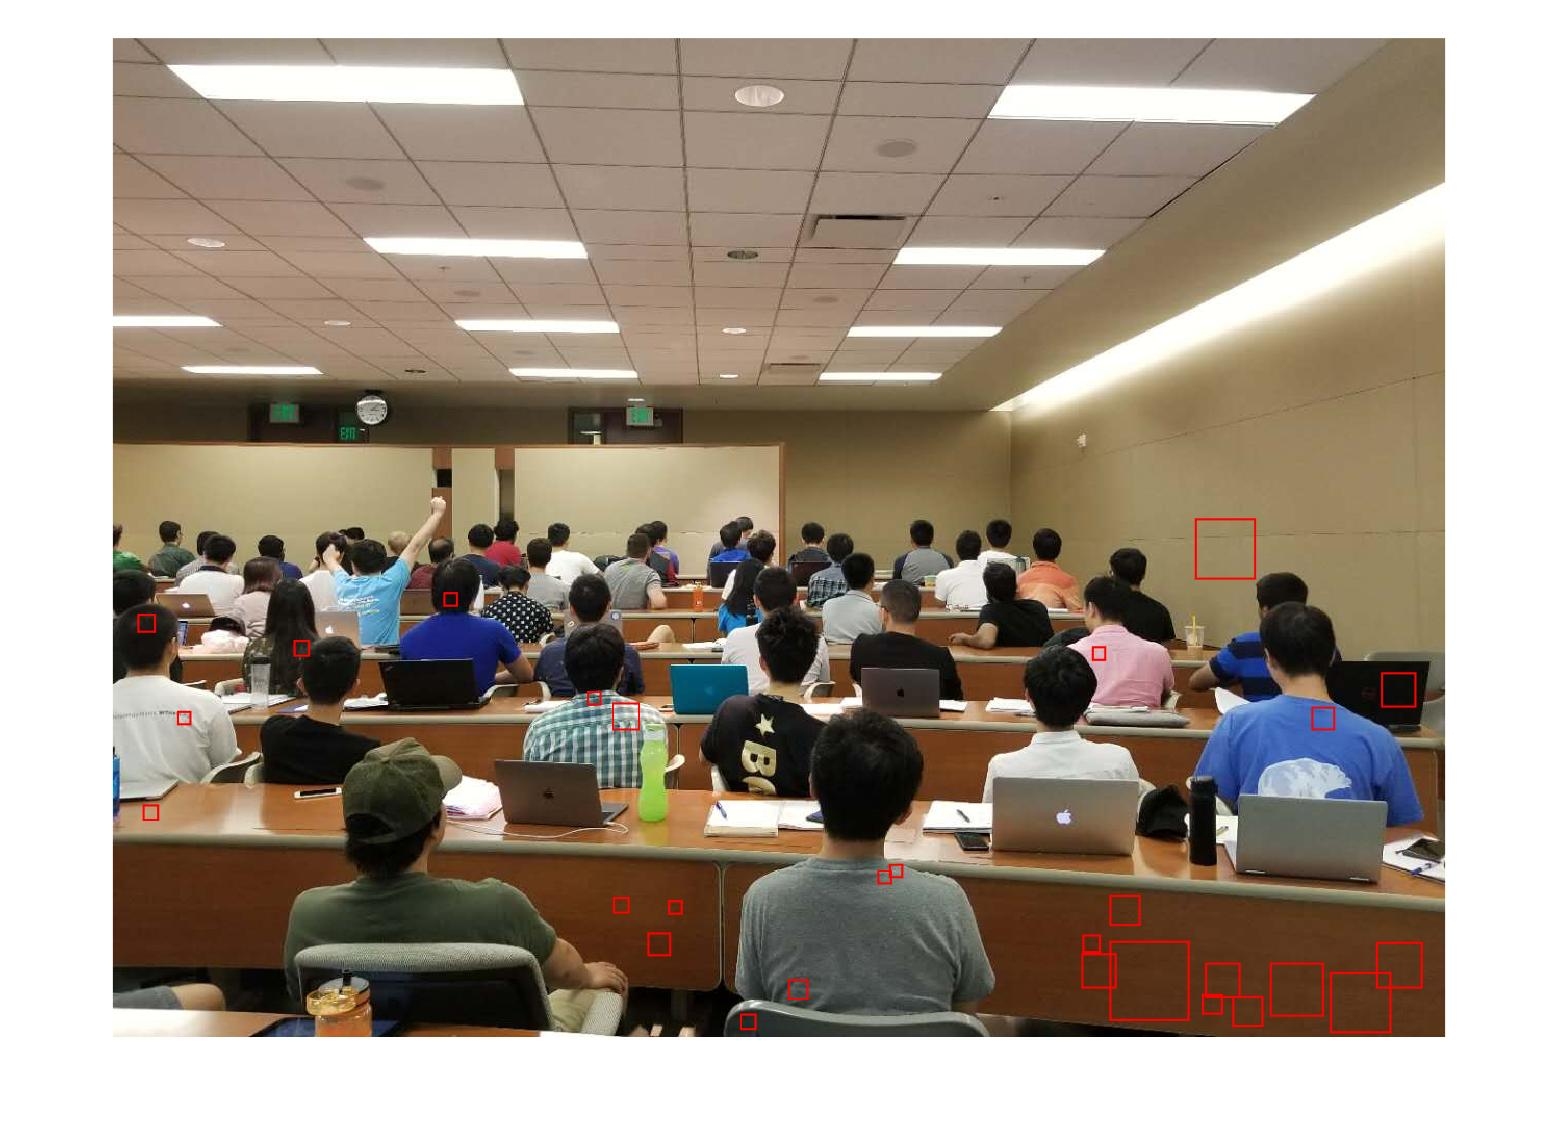
\includegraphics[width=\textwidth]{detection_nonface_1.jpg}
		\centering
		\caption{Detection result for negative sample image 1 without hard negative mining.}
		\label{11}
	\end{figure}
	\newpage\begin{figure}[ht]
		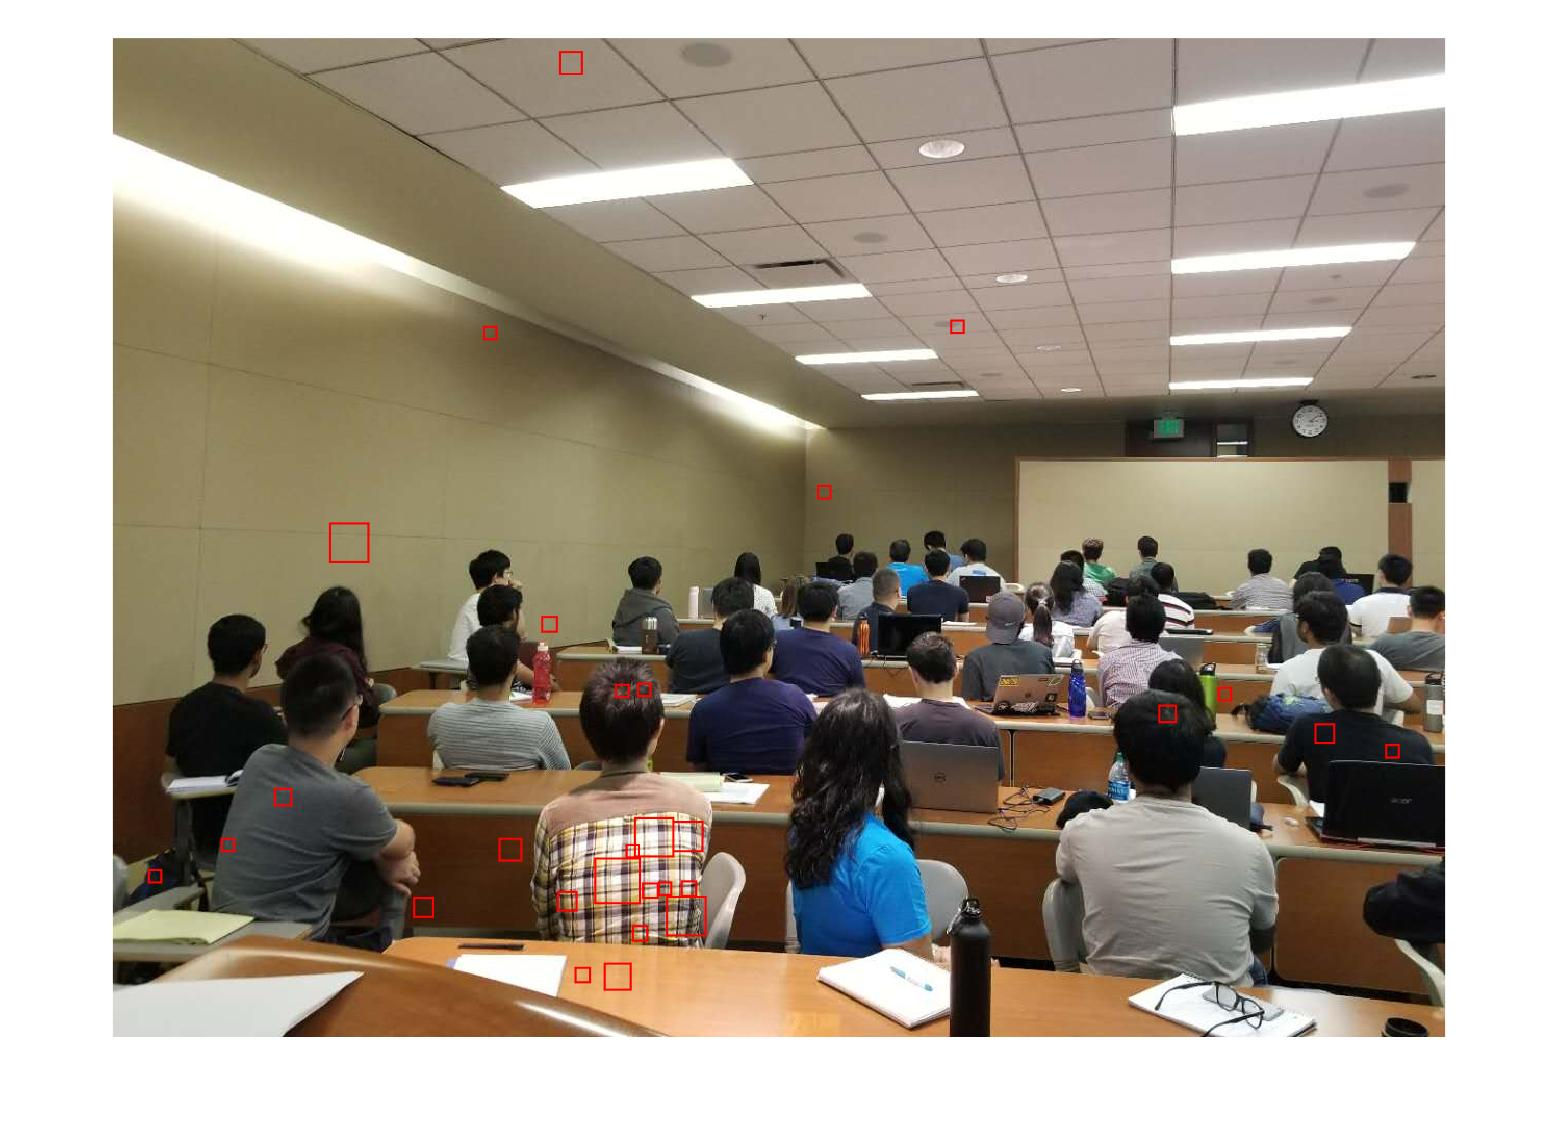
\includegraphics[width=\textwidth]{detection_nonface_2.jpg}
		\centering
		\caption{Detection result for negative sample image 2 without hard negative mining.}
		\label{12}
	\end{figure}
	\newpage\begin{figure}[ht]
		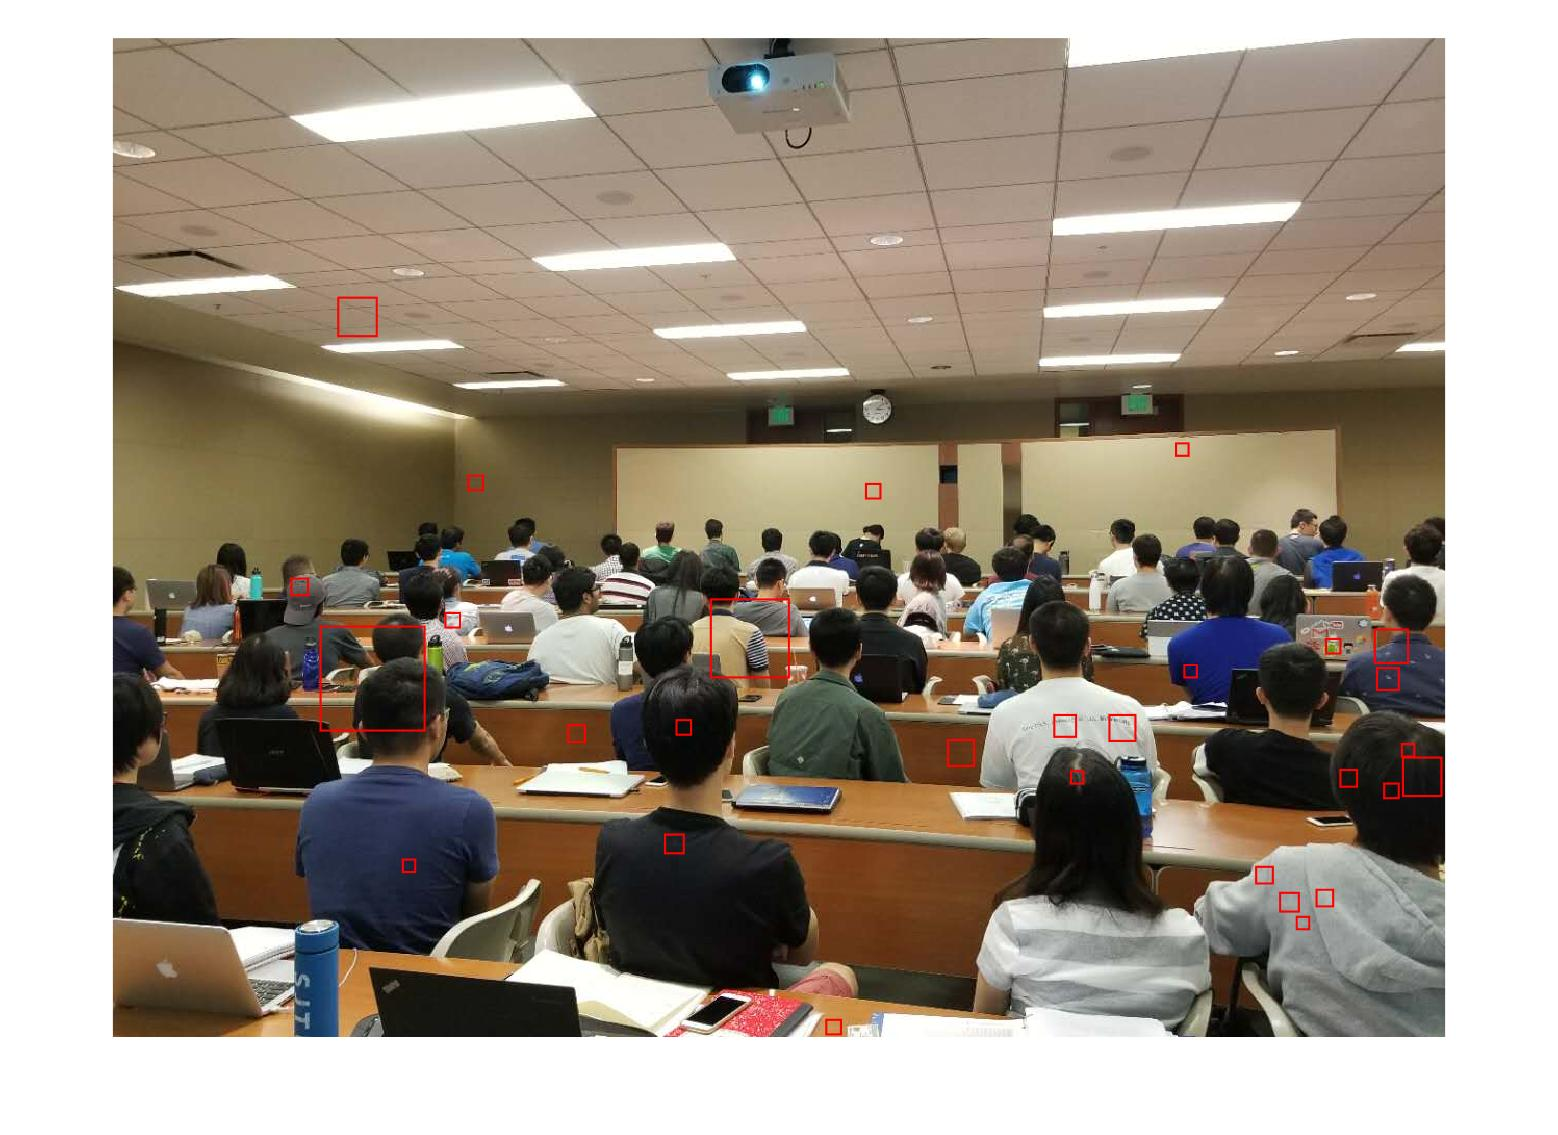
\includegraphics[width=\textwidth]{detection_nonface_3.jpg}
		\centering
		\caption{Detection result for negative sample image 3 without hard negative mining.}
		\label{13}
	\end{figure}
	(g) \textbf{Hard negative mining:} While performing detection on negative sample images, we add features of false alarms to the feature matrix in order to avoid re-computations. Re-train the classifiers from the very beginning with hard negatives added. Follow the same procedure as described in (f) to detect faces in sample images. Figure 14, 15, 16 display the detection results on positive sample images, from which we see that the number of false alarms significantly drops. However, some previously detected faces are not detected by the newly trained strong classifier. Figure 17, 18, 19 display the detection results on negative sample images. We see that there are only a few false alarms in this case, which means that hard negative mining is quite effective. \\
	\newpage\begin{figure}[ht]
		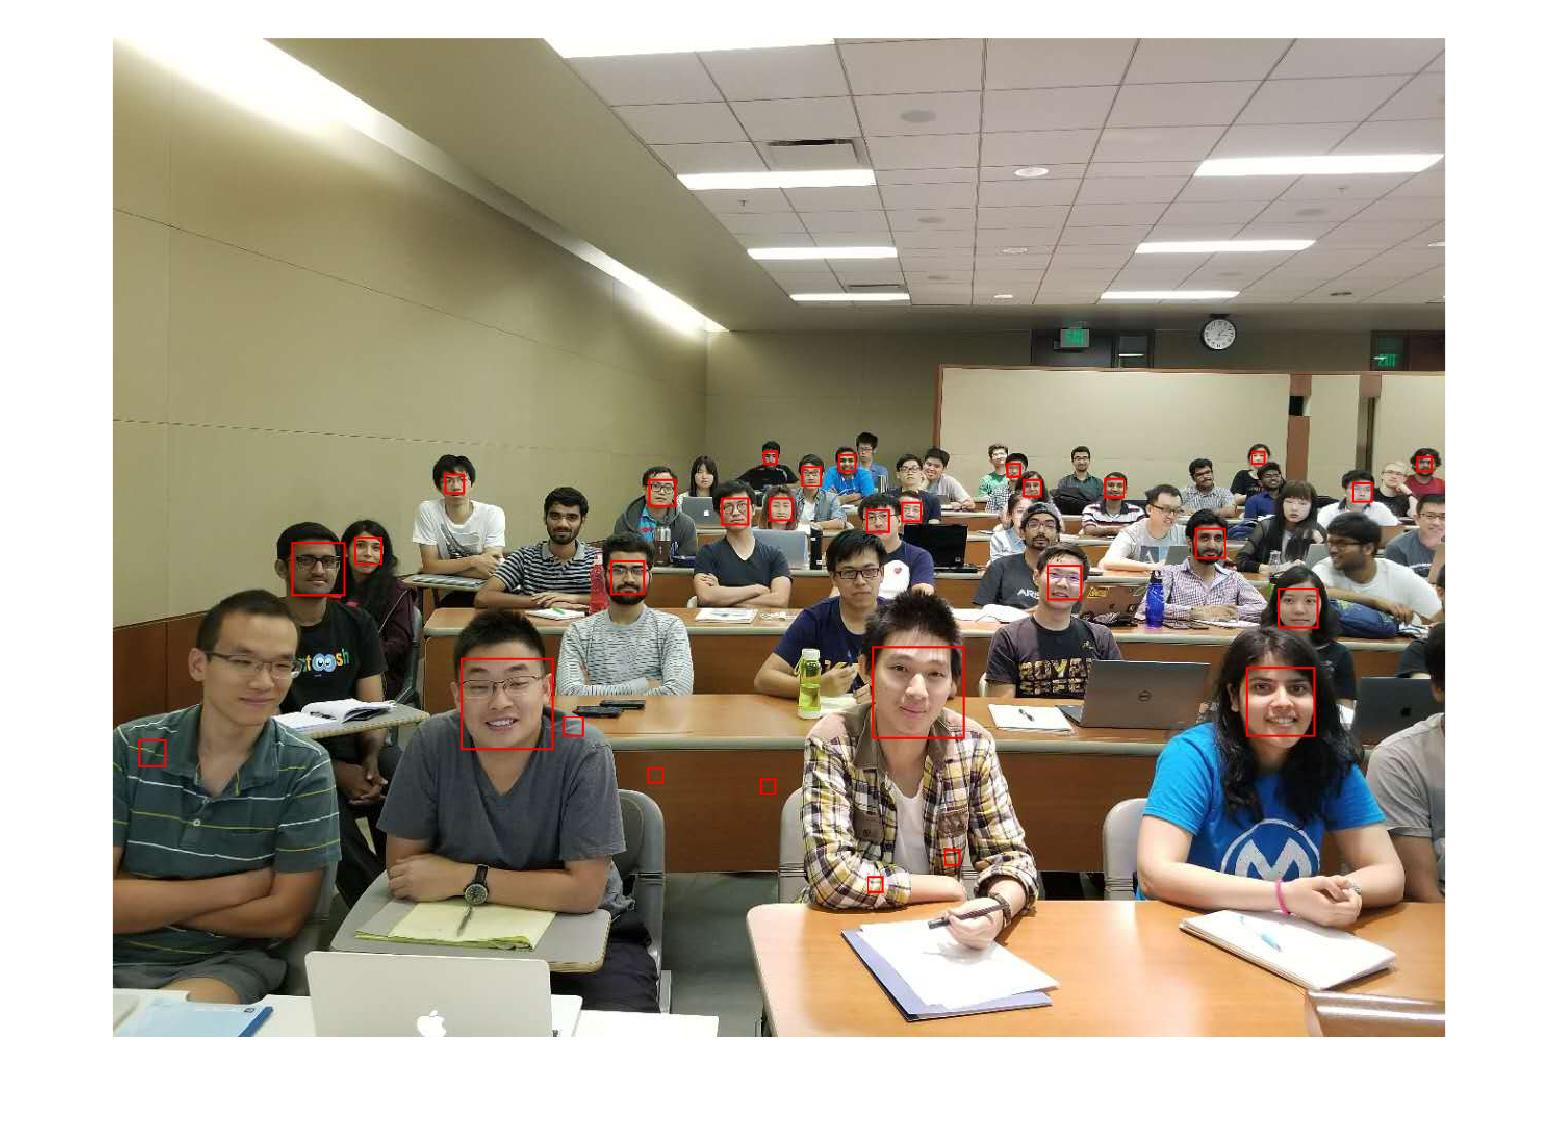
\includegraphics[width=\textwidth]{detection_face_1_hard_neg.jpg}
		\centering
		\caption{Detection result for positive sample image 1 with hard negative mining.}
		\label{14}
	\end{figure}
	\newpage\begin{figure}[ht]
		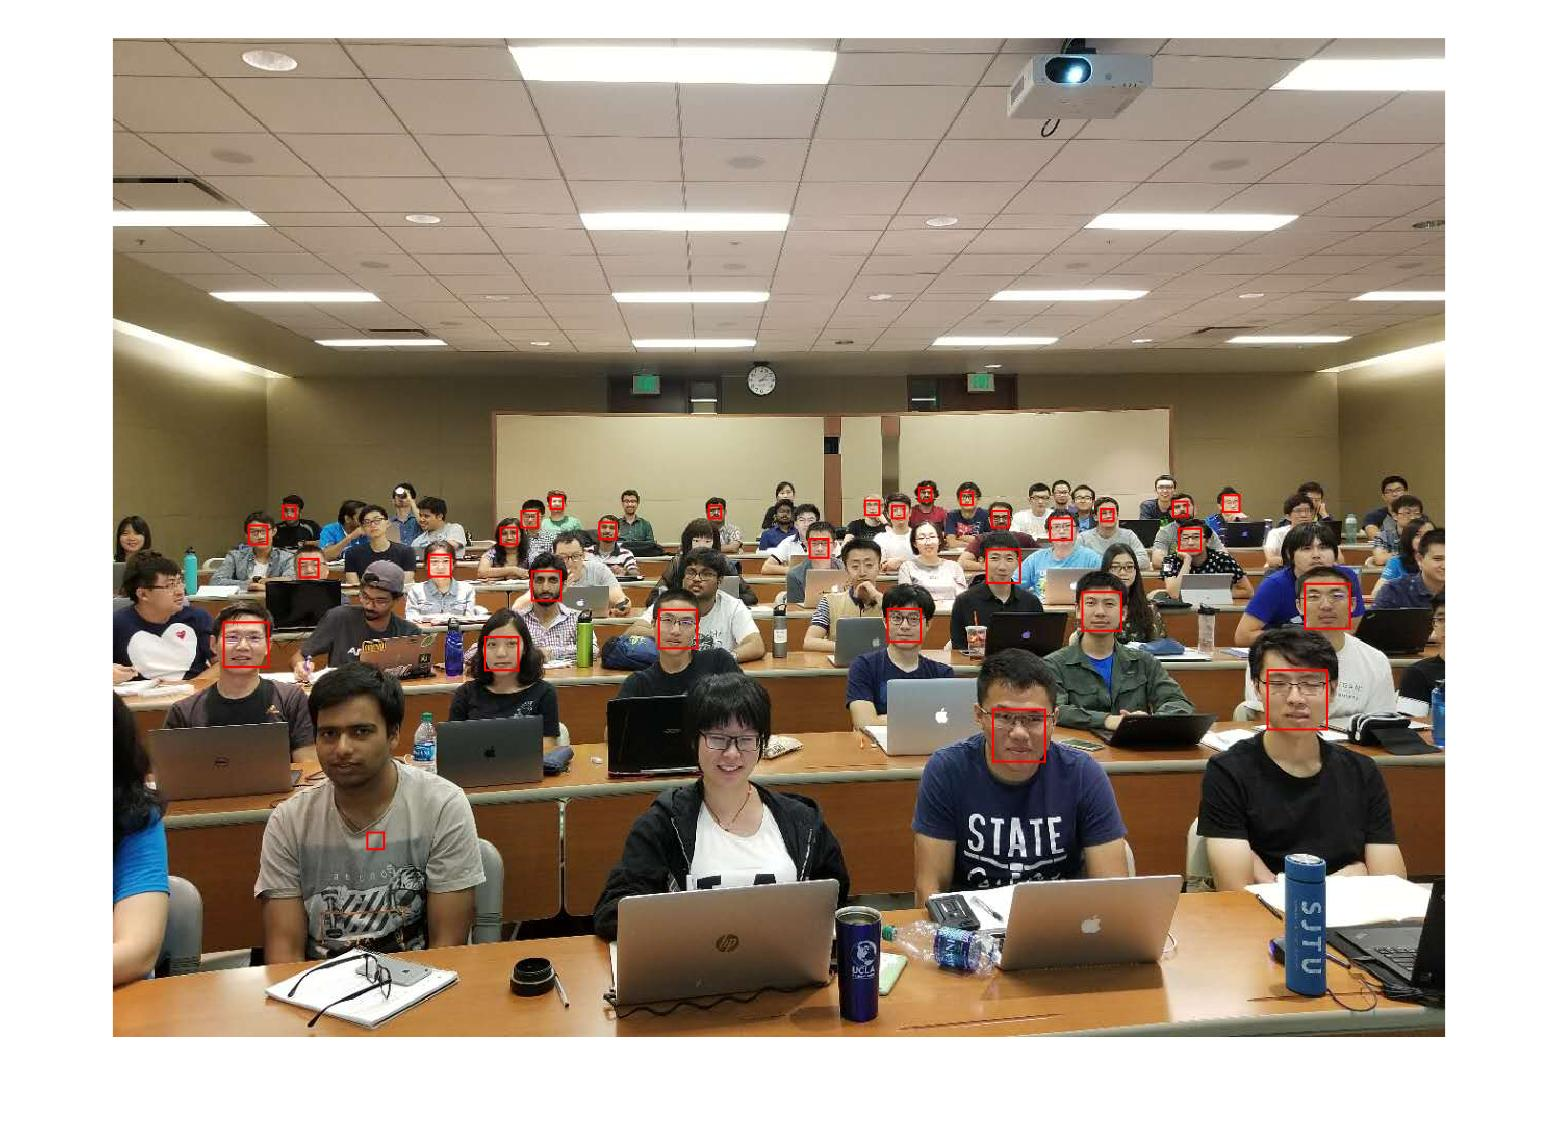
\includegraphics[width=\textwidth]{detection_face_2_hard_neg.jpg}
		\centering
		\caption{Detection result for positive sample image 2 with hard negative mining.}
		\label{15}
	\end{figure}
	\newpage\begin{figure}[ht]
		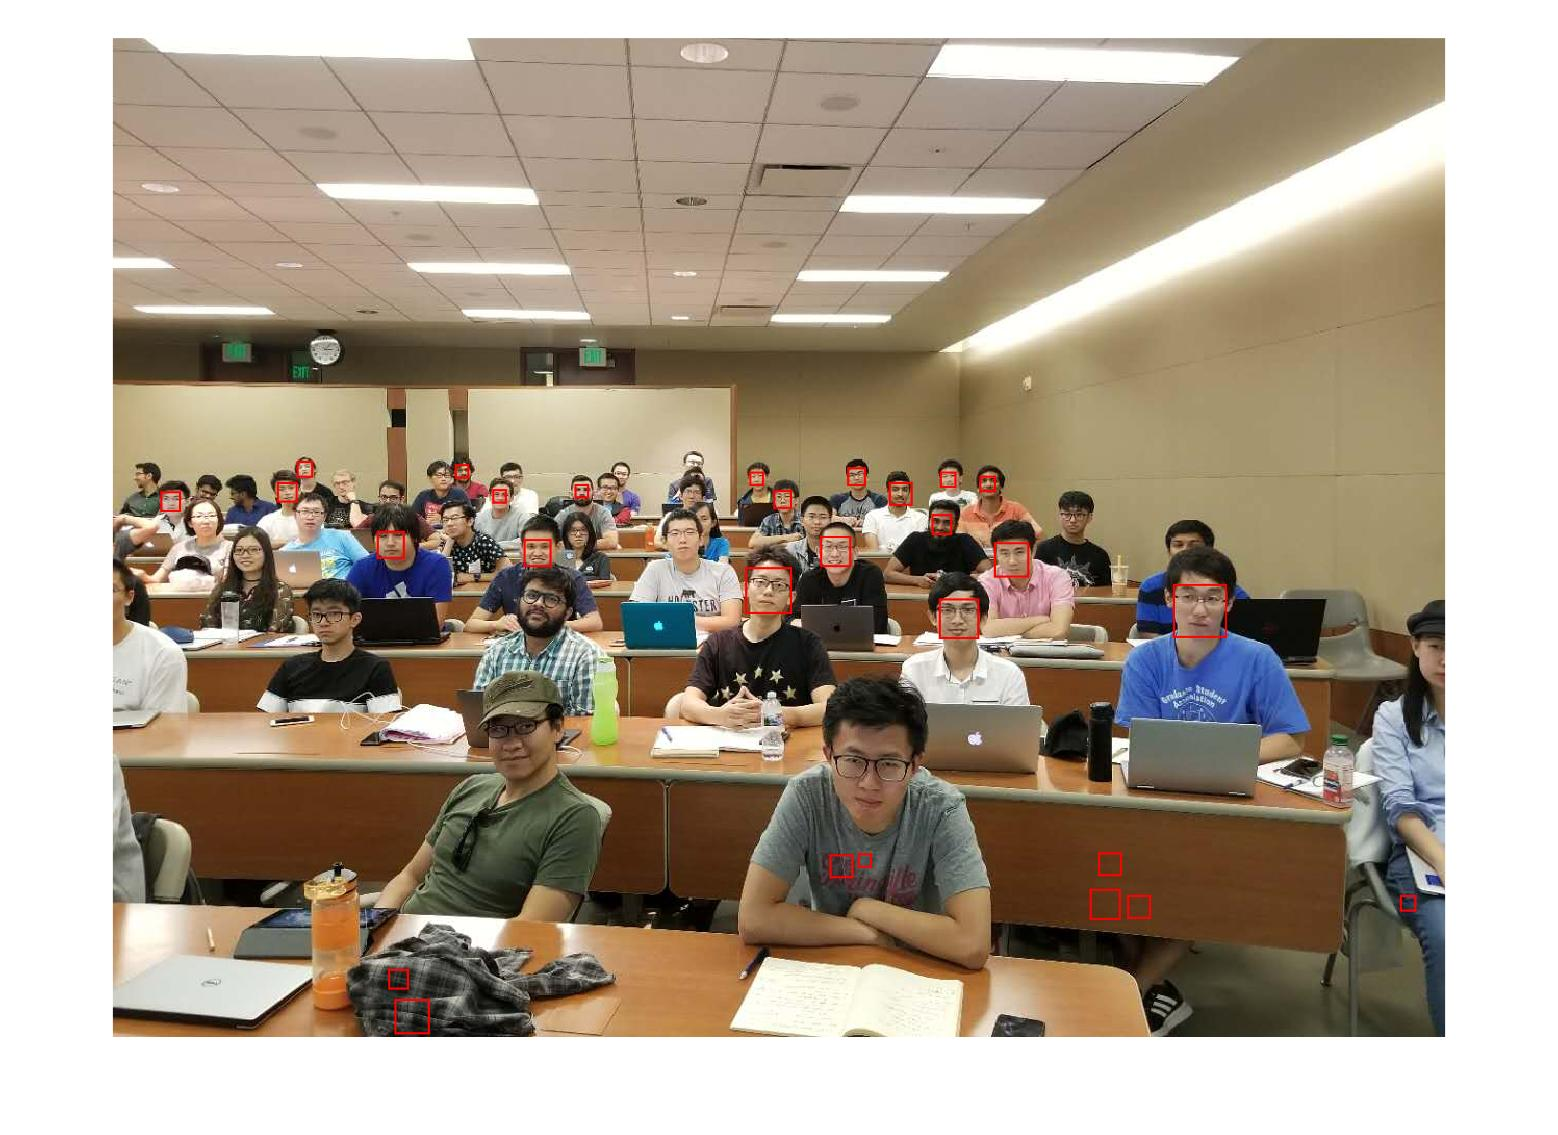
\includegraphics[width=\textwidth]{detection_face_3_hard_neg.jpg}
		\centering
		\caption{Detection result for positive sample image 3 with hard negative mining.}
		\label{16}
	\end{figure}
	\newpage\begin{figure}[ht]
		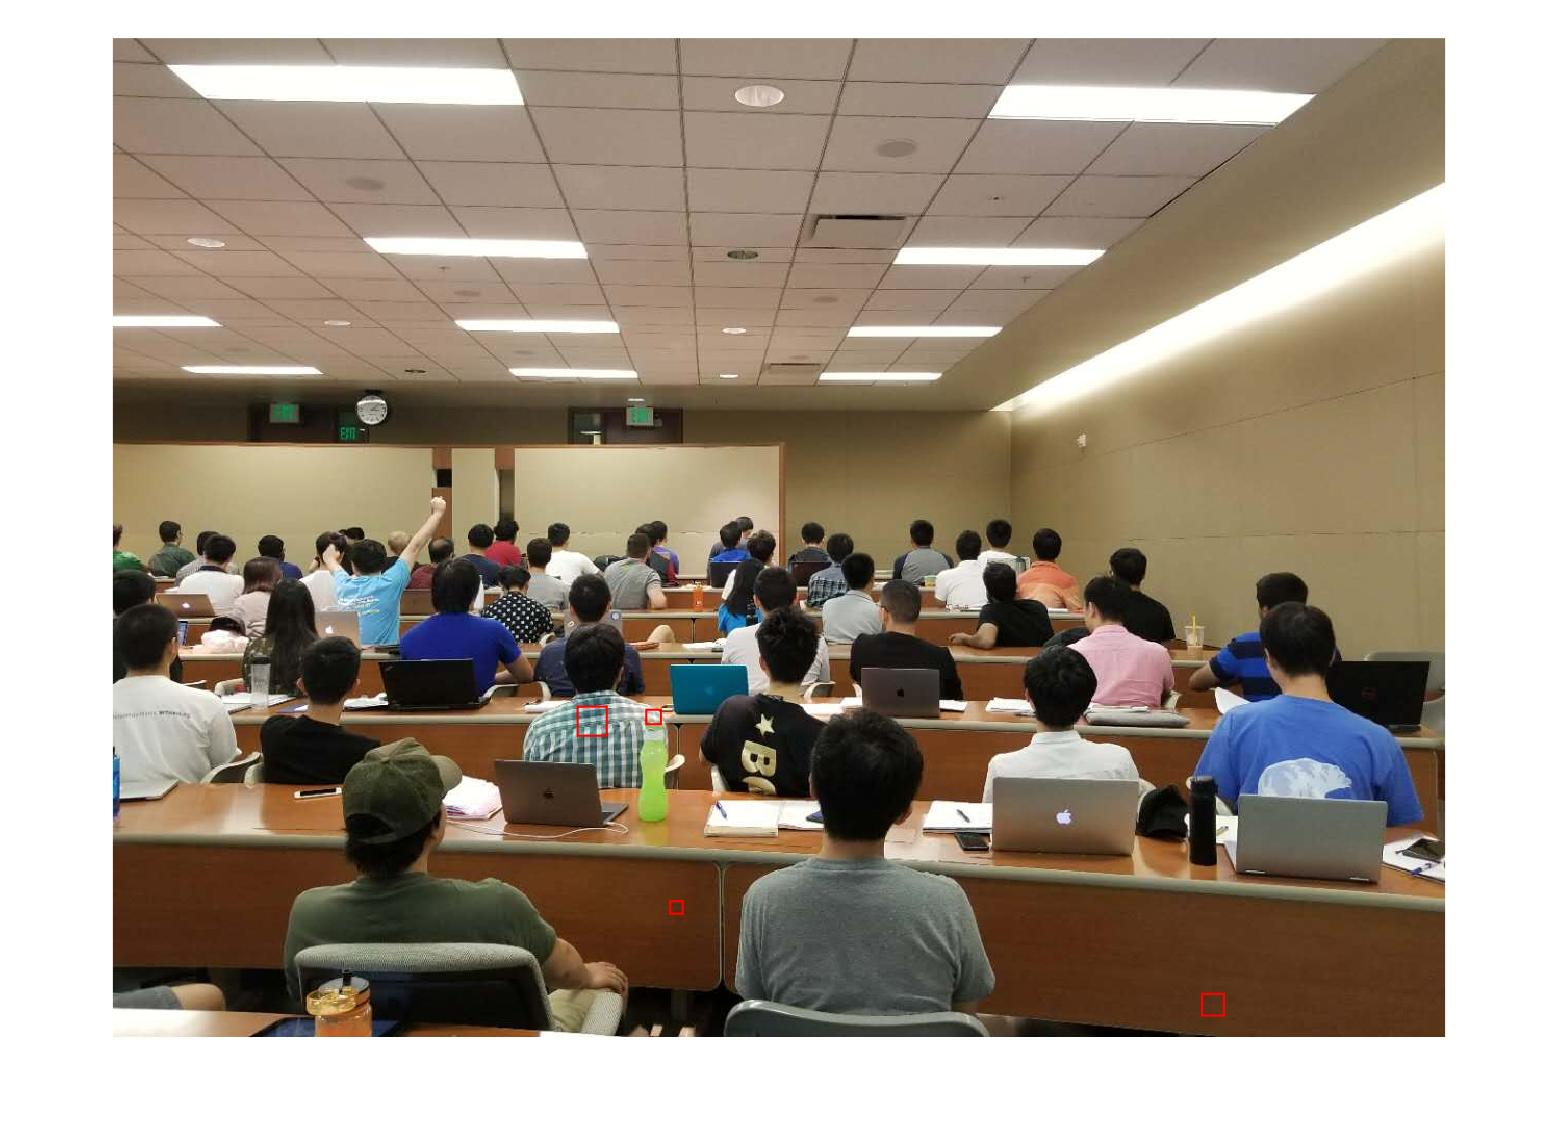
\includegraphics[width=\textwidth]{detection_nonface_1_hard_neg.jpg}
		\centering
		\caption{Detection result for negative sample image 1 with hard negative mining.}
		\label{17}
	\end{figure}
	\newpage\begin{figure}[ht]
		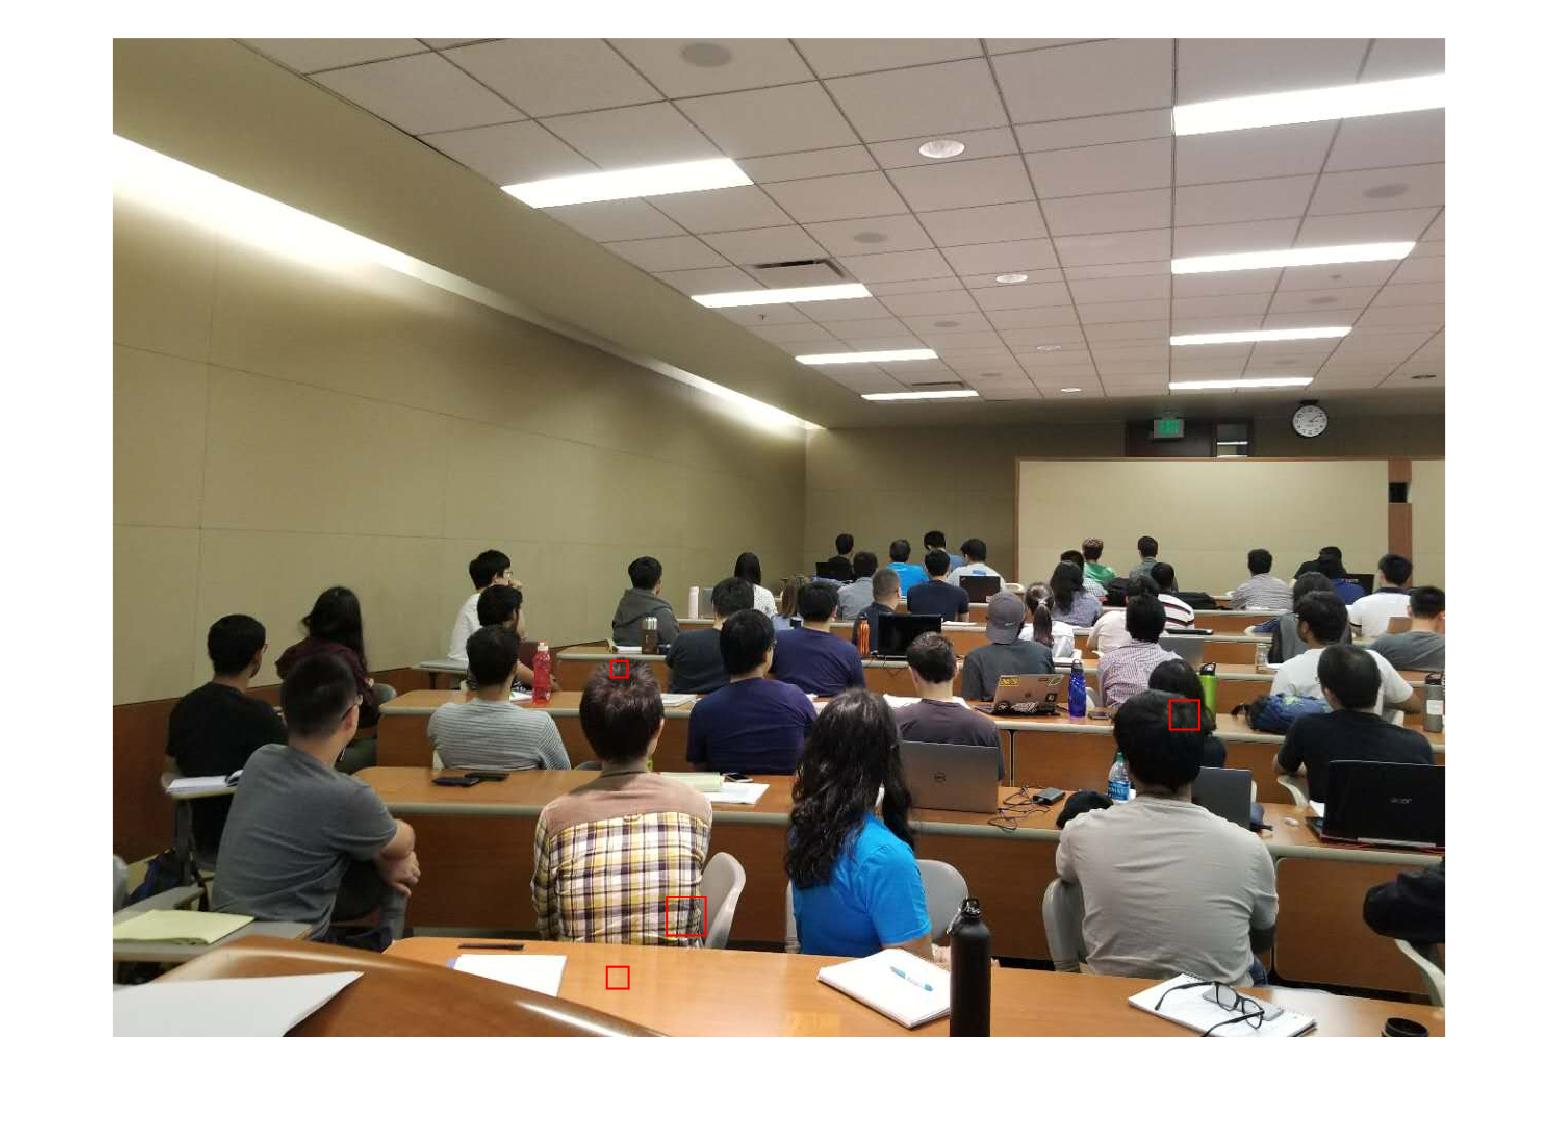
\includegraphics[width=\textwidth]{detection_nonface_2_hard_neg.jpg}
		\centering
		\caption{Detection result for negative sample image 2 with hard negative mining.}
		\label{18}
	\end{figure}
	\newpage\begin{figure}[ht]
		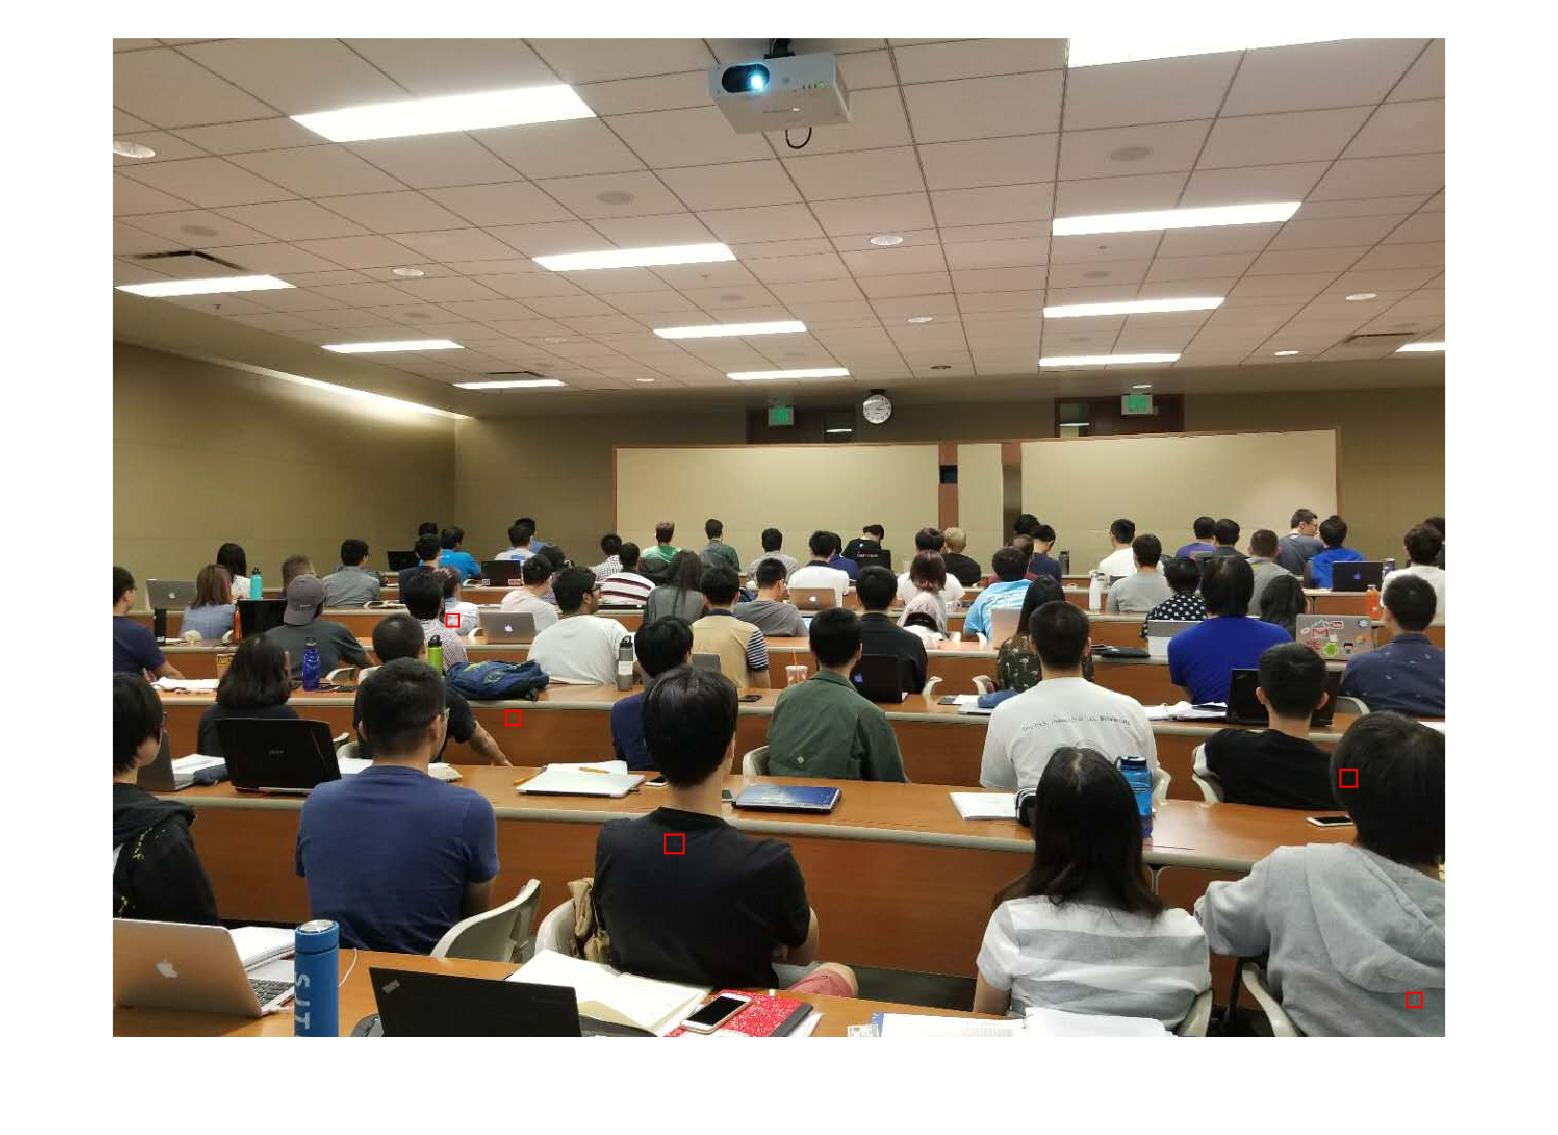
\includegraphics[width=\textwidth]{detection_nonface_3_hard_neg.jpg}
		\centering
		\caption{Detection result for negative sample image 3 with hard negative mining.}
		\label{19}
	\end{figure}

\section*{\large{Task 3: Implement RealBoost}}
Implement the RealBoost algorithm using the top $T=10,50,100$ features we choose in step (c). Our implementation of the RealBoost algorithm (with $20$ bins) turns out to be about $\times5$ faster than that of the AdaBoost algorithm. \\\\
	(h) \textbf{Histograms:} Figure 20, 21, 22 display the histograms of the positive and negative populations over $F(x)$ after running the RealBoost algorithm, for $T=10,50,100$, respectively. Like what we see in (d), as the boosting process continues, the intersection of positive and negative populations become smaller, which proves that RealBoost is also effective in our task.\\
	\begin{figure}[ht]
		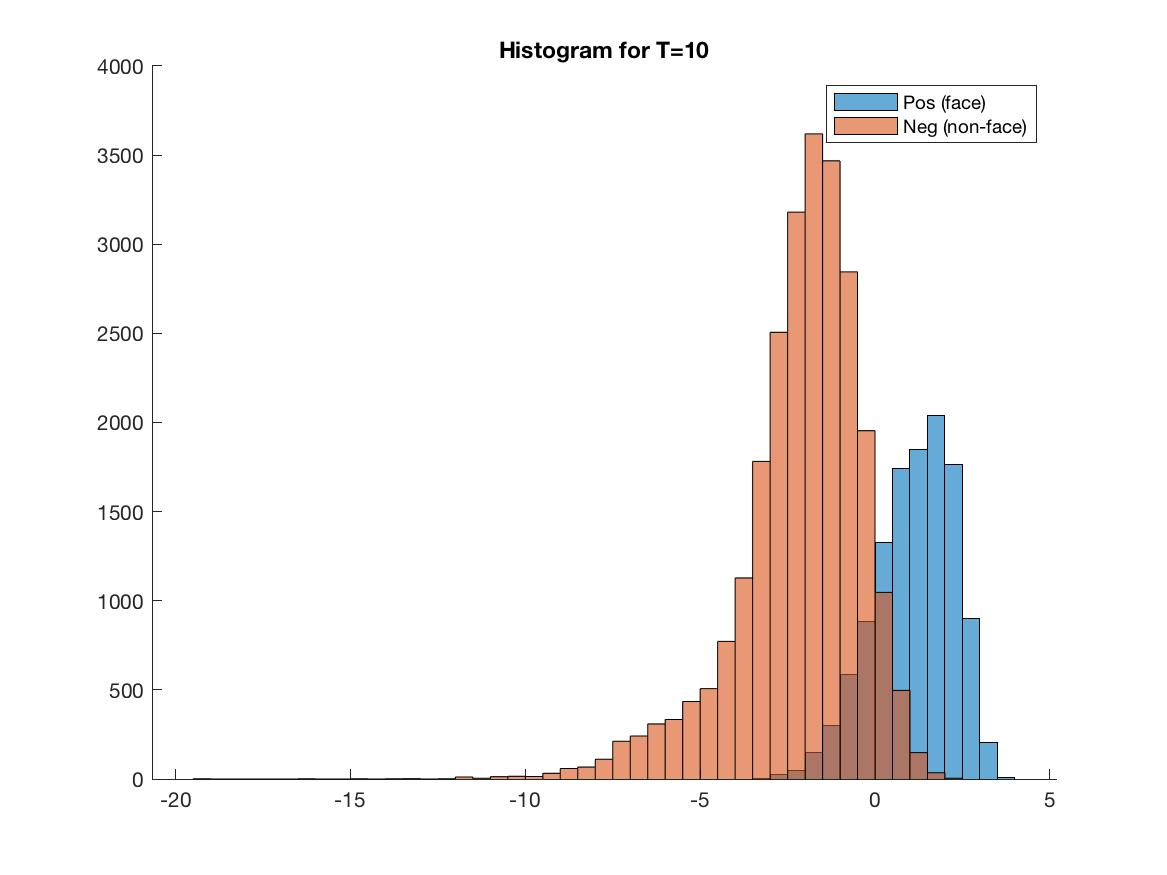
\includegraphics[scale = 0.2]{pos_neg_hist_10_real.jpg}
		\centering
		\caption{The positive and negative populations over $F(x)$ for $T=10$ (RealBoost).}
		\label{20}
	\end{figure}
	\begin{figure}[ht]
		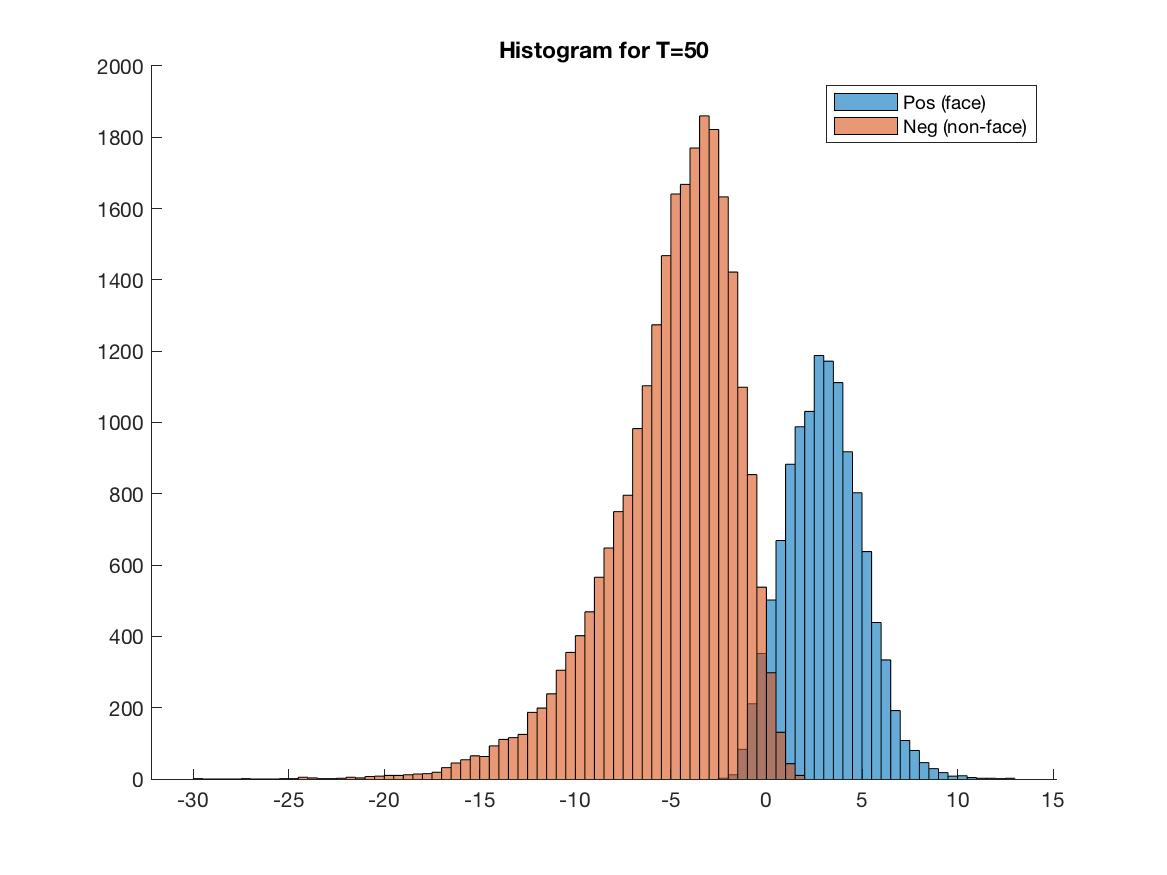
\includegraphics[scale = 0.2]{pos_neg_hist_50_real.jpg}
		\centering
		\caption{The positive and negative populations over $F(x)$ for $T=50$ (RealBoost).}
		\label{21}
	\end{figure}
	\begin{figure}[ht]
		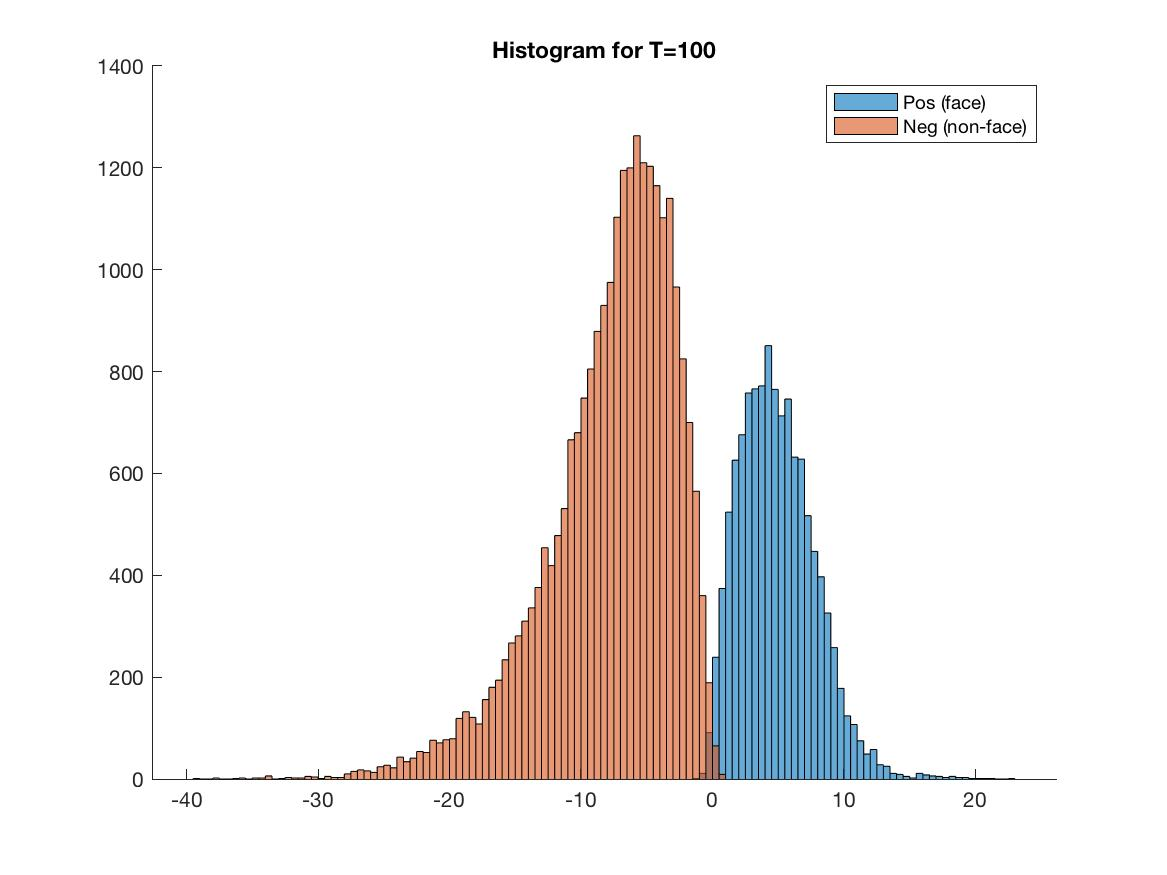
\includegraphics[scale = 0.2]{pos_neg_hist_100_real.jpg}
		\centering
		\caption{The positive and negative populations over $F(x)$ for $T=100$ (RealBoost).}
		\label{22}
	\end{figure}\\
	\newpage(i) \textbf{ROC:} Figure 23 shows the corresponding ROC curves for the histograms of $T=10,50,100$ respectively. Like what we observe in (e), the curve is much more uplifted toward the corner $(0,1)$ as $T$ becomes larger. When we compare this plot with that in (e), we also notice that RealBoost achieves a better performance than AdaBoost, which shows that using a real number voting can be better than using a binary voting.\\
	\begin{figure}[ht]
		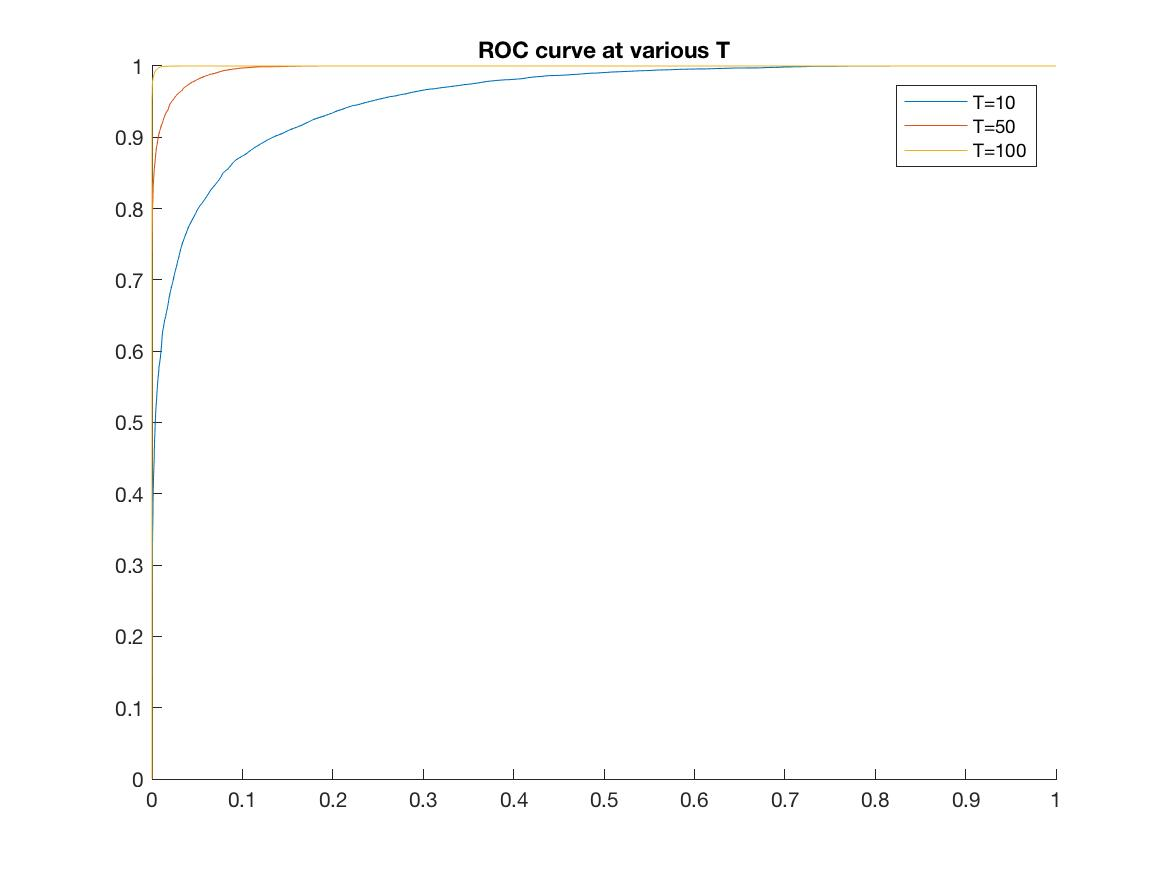
\includegraphics[scale = 0.25]{roc_real.jpg}
		\centering
		\caption{ROC curves for $T=10,50,100$ (RealBoost).}
		\label{23}
	\end{figure}\\
\end{document}